\chapter{Structure and Stability of the Mapper}
\label{chap:MapperStability}

%Even though Reeb graphs are stable with respect to perturbations of the data,
%their discrete analogues, the Mappers, are not. 
In Chapter~\ref{chap:backgroundTelescopesReeb}, we have seen how distances between Reeb graphs
can be related to each other. In this chapter, we turn the focus on studying 
the structure and defining stable distances between Mappers, which are pixelized versions of Reeb graphs.

Indeed, somewhat surprisingly, despite its success in applications, very little is
known to date about the structure of the Mapper and its stability with
respect to perturbations of the data or of the cover. Intuitively, 
as a pixelized version of the Reeb graph, the Mapper should capture
some of its topological features (branches, holes) and miss others, 
depending on how its cover is positioned. 
The stability of the structure of the Mapper, and thus the 
corresponding distance used to compare them, should also depend on this positioning.
 
%How can we quantify it?  These are the questions addressed in this chapter.
%In this chapter, we tackle this problem by proving {\em stability} results for  Mappers .

The main result of this chapter is to formalize this intuition. We show in Theorem~\ref{th:ExDgMultiNerve}
that the topological structure of the Mapper can be read off from the one of the Reeb graph through
a simple procedure. We build on this procedure to show Theorem~\ref{thm:MStab}, which states that Mappers are
actually stable when compared with an appropriate distance. 
%that we can take inspiration from this procedure to define a distance stabilizing the Mappers.
More precisely, we show that:
\begin{itemize}
\item $\Dg(\Mapper_f(X,\I))=\Dg(\Reeb_f(X))\setminus Q_{\I}$ is a bag-of-features signature of the topological structure of the Mapper,
and can be computed solely by removing points of $\Dg(\Reeb_f(X))$ that belong to a specific area $Q_{\I}$ of the plane, which only depends on the cover $\I$
(Theorem~\ref{th:ExDgMultiNerve}),
\item this signature is stable: $d_{\I}(\Dg(\Mapper_f(X,\I)),\Dg(\Mapper_g(X,\I)))\leq \|f-g\|_\infty$, where $d_{\I}$ is a distance 
depending only on $Q_{\I}$ (Theorem~\ref{thm:MStab}). 
\end{itemize}

The area $Q_{\I}$ is a direct measure of the approximation quality of the Mapper: 
if $\I$ contains large intervals, then many points of $\Dg(\Reeb_f(X))$ will be included in $Q_{\I}$, and  
thus the Mapper is going to be a very rough approximation of the Reeb graph. This is formalized in Corollary~\ref{cor:Reeb_approx}.

We end the chapter by showing that any Mapper %$\Mapper_f(X,\I)$ 
is actually isomorphic to a specific Reeb graph, whose connection to the one that the Mapper is approximating
can be controlled in both the bottleneck (Theorem~\ref{th:MultiNerveCover}) and functional distortion distance (Theorem~\ref{th:dfd}).

To prove all of these results, we use an intermediate construction called the {\em MultiNerve Mapper},
which is a slight, and somehow natural, extension of the usual Mapper.

%The stable descriptor $\Dg(\Mapper_f(X,\I))$ require to know $\Dg(\Reeb_f(X))$ to be computed. Even though
%it can be approximated, 



%that can be computed directly. It takes the form of the extended persistence diagram of a particular Reeb graph which 
%is isomorphic to the Mapper. 
%Even though this second signature is instable, it enjoys a convergence result both in the bottleneck and functional distortion distance  

%
%new mathematical object to summarize the topological structure of a pair $(X,f:X\to\R)$. 
%Its construction depends on the choice of a cover~$\I$ of the
%image of $f$ by open sets. Pulling back~$\I$ through $f$ gives an
%open cover of the domain $X$. This cover may have some elements that
%are disconnected, so it is refined into a connected cover by splitting
%each element into its various connected components. Then, the Mapper
%is defined as the nerve of the connected cover, having one vertex per
%element, one edge per pair of intersecting elements, and more
%generally, one $k$-simplex per non-empty ($k+1$)-fold
%intersection. From a philosophical point of view, the Mapper can be
%thought of as a {\em pixelized version} of the Reeb graph, where the
%resolution is prescribed by the cover~$\I$. 

%As a simple alternative to the Reeb graph, the Mapper has been the
%object of much interest by practitioners in the data sciences. It has
%played a key role in several success stories, such as the
%identification of a new subgroup of breast
%cancers~\cite{Nicolau11}, or the elaboration of a new
%classification of player positions in the NBA~\cite{NBA}, due to its ability to
%deal with very general functions and datasets. Meanwhile,
%it has become the flagship component in the software suite developed
%by Ayasdi, a data analytics company founded in the late 2000's whose
%interest is to promote the use of topological methods in the data
%Sciences. 

\paragraph*{Plan of the Chapter.} We first give properties of Mappers computed with scalar-valued functions in Section~\ref{sec:1Dmapper}. 
We then detail a variant therof, the {\em MultiNerve Mapper},
in Section~\ref{sec:MultiNerveMapper}. Next, we show how the topological structure of the (MultiNerve) Mapper can actually be derived
from the one of the Reeb graph in Section~\ref{sec:structure}. This allows us to define an adequate and computable pseudometric to compare the
(MultiNerve) Mappers and provide stability results in Sections~\ref{sec:Stab_func} and~\ref{sec:Stab_cover}. Finally, we use the telescope operators of
Section~\ref{sec:operator} to provide a convergence result of the (MultiNerve) Mapper to the Reeb graph in the 
functional distortion distance in Section~\ref{sec:stabdfd}. 

%\paragraph*{Publications.} This chapter corresponds to the articles~\cite{Carriere15c} and~\cite{Carriere16}.


\section{Mappers for scalar-valued functions}
\label{sec:1Dmapper}

We begin the chapter with some remarks on Mappers computed with scalar-valued functions.
In particular, we show that, for specifics covers of the real line called {\em gomics}, these 1-dimensional Mappers
have multigraph structures. 

\paragraph*{Interval cover.} Let $Z$ be a subset of $\R$, equipped
with the subspace topology. A subset $U\subseteq Z$ is an {\em interval of $Z$} 
if there is an interval $I$ of $\R$ such that
$U=I\cap Z$. Note that $U$ is open in $Z$ if and only if $I$ can be
chosen open in $\R$.  A cover $\I$ of $Z$ is an {\em interval cover}
if all its elements are intervals. In this case, $\End(\I)$
denotes the set of all of the interval endpoints. Finally, the
{\em granularity} of $\I$ is the
supremum of the lengths of its elements, i.e. it is the quantity $\text{sup}_{I\in\I}\ |I|$ where
$|I|=\sup(I)-\inf(I)\in\R\cup\{+\infty\}$.

\begin{lem}\label{lem:minimal-cover_1-dim}
No more than two elements of an open minimal interval cover can intersect at a time.
\end{lem}
%
\begin{proof}
Assume for a contradiction that there are $k\geq 3$ elements
of $\I$: $U_1, \cdots, U_k$, that have a non-empty common intersection. For
every $i$, fix an open interval $I_i$ of $\R$ such that $U_i=I_i\cap Z$. Up to
a reordering of the indices, we can assume without loss of generality
that $I_1$ has the smallest lower bound and $I_2$ has the largest
upper bound. Since $I_1\cap I_2 \supseteq U_1\cap U_2 \neq\emptyset$,
the remaining intervals satisfy $I_i\subseteq I_1\cup I_2$. In
particular, we have $U_3= I_3\cap Z\subseteq (I_1\cup I_2)\cap Z =
(I_1\cap Z)\cup (I_2\cap Z) = U_1\cup U_2$, so the cover $\I$ is not
minimal.
\end{proof}
%
\begin{lem}
If $Z$ is $\R$ or a compact subset thereof, any cover $\I$
of $Z$ has a minimal subcover.
\end{lem}
%
\begin{proof}
When $Z$ is compact, there exists a subcover $\J$ of $\I$ that has
finitely many elements.  Any subcover of $\J$ with the minimum number of
elements is then a minimal cover of $Z$.

When $Z=\R$, the same argument applies to any subset of the form $[-n, n]$, $n\in \N$. 
Then, a simple induction on $n$ allows us to build a minimal subcover of $\I$. 
\end{proof}

\paragraph*{Gomics.} From now on, unless otherwise stated, all covers of $Z\subseteq \R$
will be generic, open, minimal, interval covers ({\em gomics} for
short). Given such a cover~$\I$, the proper subset $\Ipr$ (as defined in Section~\ref{sec:Mapperdef}) of any
interval $I\in\I$ is itself an interval of~$Z$ since $\I$ is generic, therefore we call it
the {\em proper subinterval} of~$I$.
Moreover, Lemma~\ref{lem:minimal-cover_1-dim} yields a total order on the intervals of~$\I$, 
so each one of them partitions into subintervals as follows:
%
\begin{equation}\label{eq:U_partition}
I=\Imi\sqcup\Ipr\sqcup\Ipl,
\end{equation}
%
where $\Imi$ is the intersection of $I$ with the element right below it in the cover ($\Imi=\emptyset$ if that element does not exist), 
and where $\Ipl$ is the intersection of $I$ with the element right above it ($\Ipl=\emptyset$ if that element does not exist). 



\paragraph*{Mappers computed with gomics.} 
Let $X$ be a topological space and $f:X\rightarrow\R$ be a Morse-type function, whose image is covered by the cover $\I$. 
If $\I$ is a gomic, then the Mapper $\Mapper_f(X,\I)$ has a
natural 1-dimensional stratification since no more than two intervals
can intersect at a time by Lemma~\ref{lem:minimal-cover_1-dim}. Hence,
in this case, it has the structure of a (possibly infinite) combinatorial graph
and therefore has trivial homology in dimension 2 and above.
%Moreover, it comes equipped with a function defined on its nodes, as explained in the following definition:

%\begin{defin}\label{def:arbitfunc}
%Let $X$ be a topological space, $f:X\rightarrow\R$ a continuous
%function, $\I=\{I_\alpha\}_{\alpha\in A}$ a gomic of $\im(f)$ and $\V=\{V^i_\alpha\}_{\substack{1\leq i \leq c(\alpha), \alpha\in A}}$ the associated
%connected pullback cover. 
%Then we define $f_{\I}:\Mapper_f(X,\I)\rightarrow\R$ as the piecewise-linear extension of the function defined
%on the nodes of $\Mapper_f(X,\I)$ by
%$V_\alpha^i\mapsto{\rm mid}(\tilde I_\alpha),$
%where ${\rm mid}(\tilde I_\alpha)$ is the midpoint of the proper subinterval $\tilde I_\alpha$ of $I_\alpha$.
%\end{defin}

%By construction, $f_{\I}$ is a Morse-type function, whose set of critical values is $\Crit(f_{\I})=\{{\rm mid}(\tilde I)\,:\,I\in\I\}$. 
%As such, its extended persistence diagram $\Dg(f_{\I})$ and levelset zigzag persistence barcode $\DgZZ_0(f_{\I})$ are well-defined,
%and they both encode the topological structure of the Mapper.
%Note that $f_{\I}$ is somewhat arbitrary, in that any function preserving the order of the intervals of $\I$
%would carry the same information in its persistence diagram. 

%We will circumvent this issue in Section~\ref{sec:MultiNerveSign},
%where we define a canonical persistence diagram for the Mapper by pruning $\Dg(\tilde f)$.


















%%%%%%%%%
\section{MultiNerve Mapper}
\label{sec:MultiNerveMapper}

In this section, we define a slight modification of the Mapper called the {\em MultiNerve Mapper},
which can be easily related to the Mapper---see Corollary~\ref{cor:projMNonM}, and whose analysis is more natural to handle. 


\paragraph*{Simplicial Posets.}
The MultiNerve Mapper construction is based on {\em multinerves}, which are specific {\em simplicial posets}.

\begin{defin}[\cite{Verdiere12}]
A \emph{simplicial poset} is a partially ordered set $(P,\preceq)$, whose elements are called \emph{simplices}, such that:

\begin{itemize}
\item[\rm (i)] $P$ has a least element called $0$ such that $\forall p\in P$, $0\preceq p$;
\item[\rm (ii)] $\forall p\in P$, $\exists d\in\mathbb{N}$ such that the lower segment 
$[0,p]=\{q\in P\,:\,q\preceq p\}$ is \emph{isomorphic} to the
set of simplices of the standard $d$-simplex with the inclusion as partial order,
where an isomorphism between posets is a bijective and order-preserving function.
\end{itemize}
\end{defin}

Simplicial posets are extensions of simplicial complexes: while every
simplicial complex is also a simplicial poset (with inclusion as
partial order and $\emptyset$ as least element), the converse is not
always true as different simplices may have the same set of vertices.
However, these simplices cannot be faces of the same
higher-dimensional simplex, otherwise $\rm (ii)$ would be false. See
Figure~\ref{fig:PosetExample} for an example of a simplicial poset
that is not a simplicial complex.

%%%
\begin{figure}[t] 
\begin{center}
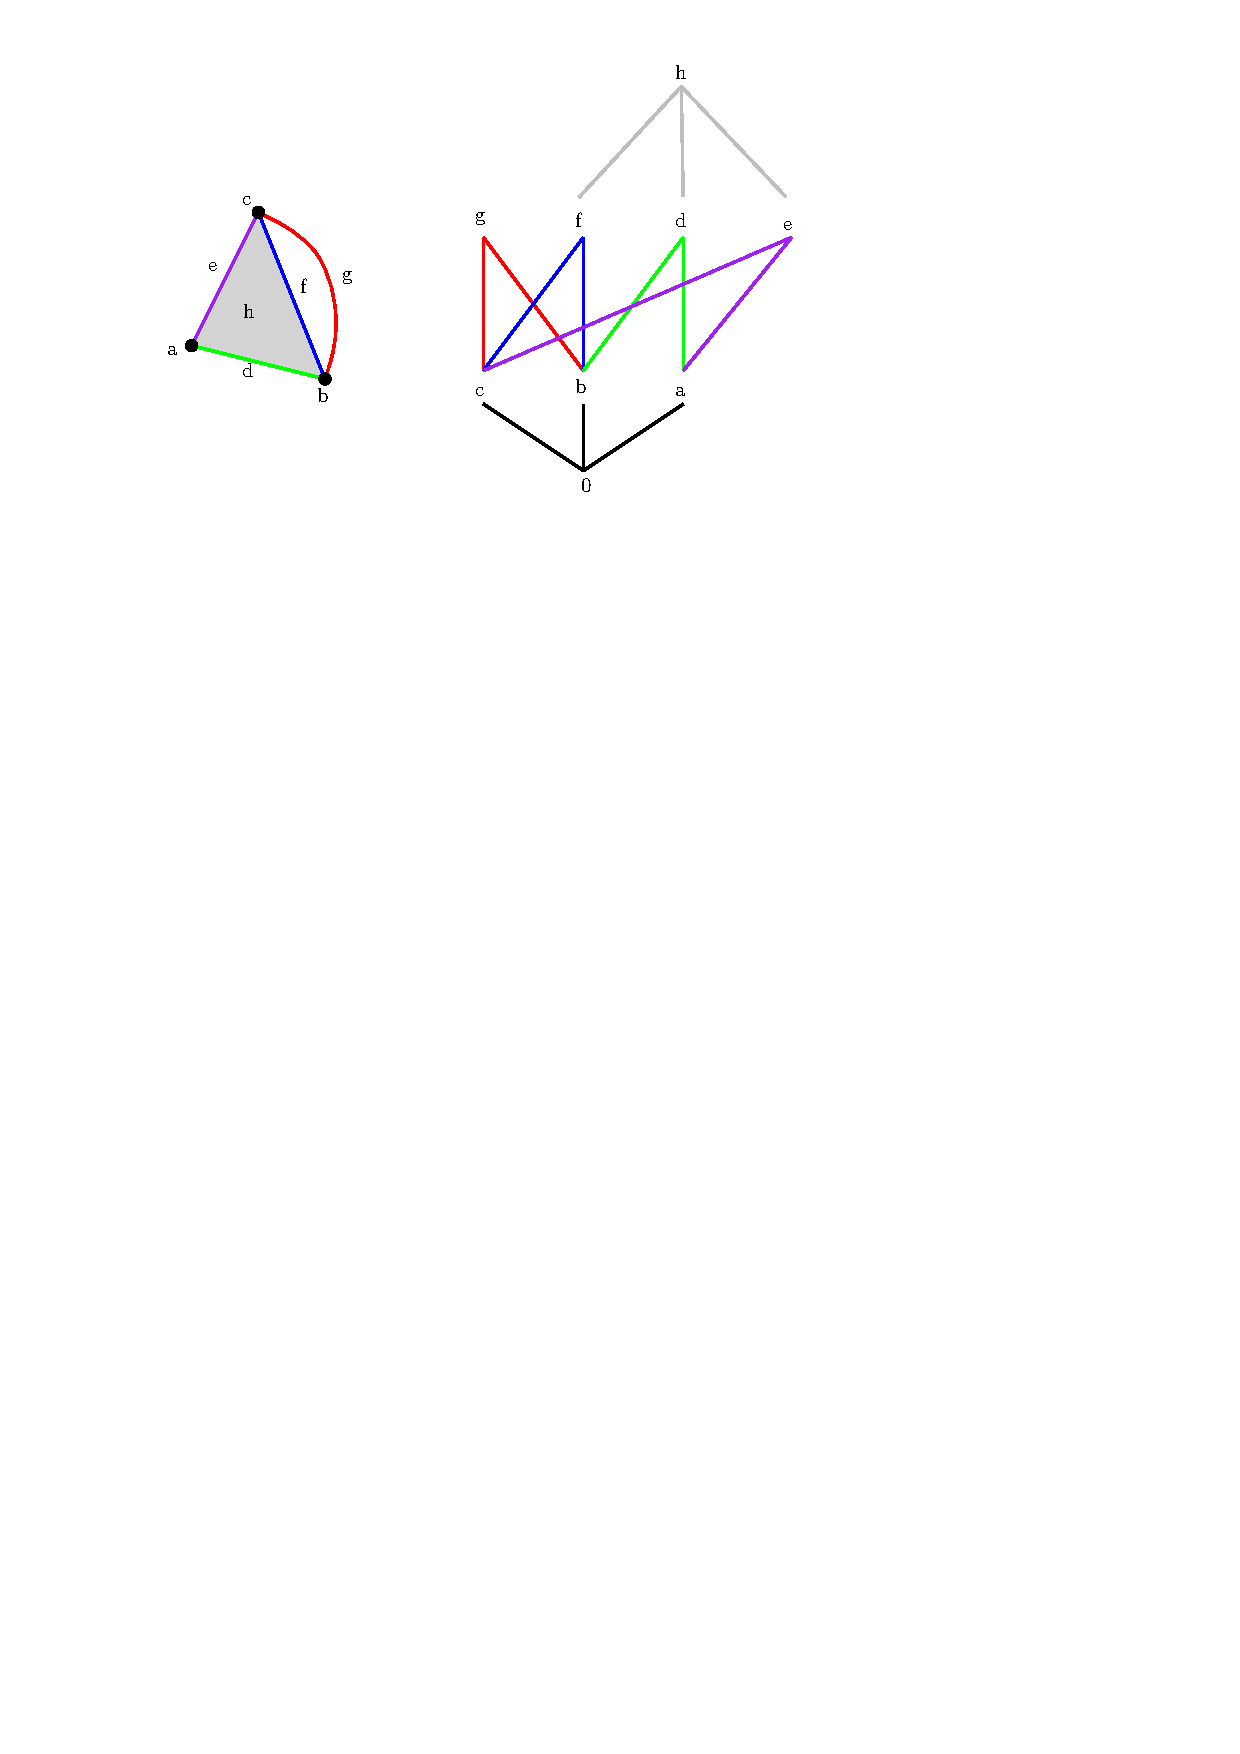
\includegraphics[height = 5cm]{figures/PosetExample}\hspace{3mm}
\caption[Simplicial poset]{\label{fig:PosetExample} Left: A simplicial poset that is not a 
simplicial complex. Indeed, edges $f$ and $g$ have the same vertices ($b$ and $c$). 
Right: The corresponding Hasse diagram showing the partial order on the simplices. Note that $f,g$
cannot be part of the same 2-cell. \vspace{-4mm}}
\end{center} 
\end{figure}

\paragraph*{Multinerve.} Given a cover $\U$ of $X$, the nerve is extended
to a simplicial poset as follows:

\begin{defin}
Let $\U=\{U_\alpha\}_{\alpha\in A}$ be a cover of a topological space $X$.
The \emph{multinerve $\M(\U)$}
is the simplicial poset defined by:
\[
\M(\U)=\left\{\left(\{\alpha_0, \cdots, \alpha_k\} ,C\right)\,:\, \bigcap_{i=0}^k 
U_{\alpha_i}\neq\emptyset\text{ and }C\text{ is a connected component of }\bigcap_{i=0}^k U_{\alpha_i}\right\}.
\]
\end{defin}

The proof that this set, together with the least element $(\emptyset,\bigcup_{\alpha\in A} U_\alpha)$
and the partial order $(F,C)\preceq(F',C')\Leftrightarrow F\subseteq F'\ \text{and}\ C'\subseteq C$, 
is a simplicial poset, can be found in \cite{Verdiere12}.
Given a simplex $(F,C)$ in the multinerve of a cover, its \textit{dimension}
is $\card(F)-1$. 
The dimension of the multinerve of a cover is the maximal dimension of
its simplices.  Given two simplices $(F,C),(F',C')$, the pair $(F,C)$ is a
{\em face} of $(F',C')$ if $(F,C)\preceq (F',C')$.  
%We also denote by $V(p)$ the
%set of vertices that are in the lower segment of $p$.


\paragraph*{MultiNerve Mapper.} Given a connected pullback cover~$\V$, we extend the Mapper by using the
multinerve $\MNerve(\V)$ instead of $\Nerve(\V)$.  This variant will
be referred to as the MultiNerve Mapper in the following.

\begin{defin}
Let $X,Z$ be topological spaces, $f:X\rightarrow Z$ be a continuous function,
$\U$ be a cover of $\im(f)$ and $\V$ be the associated connected pullback cover.

Then, the \emph{MultiNerve Mapper} of $X$ is $\MMapper_f(X,\U)=\mathcal{M}(\V)$.  
\end{defin}

See Figure~\ref{fig:mmappervsmappertorus} for an illustration.  For
the same reasons as Mapper, when $Z=\R$ and $\I$ is a gomic of
$\im(f)$, the MultiNerve Mapper $\MMapper_f(X,\I)$ is a (possibly infinite) combinatorial multigraph
having trivial homology in dimension 2 and above. 
%and it comes equipped with a piecewise-linear function
%$f_{\I}:\MMapper_f(X,\U)\rightarrow\R$ defined as in
%Definition~\ref{def:arbitfunc}.  
Contrarily to the Mapper, the MultiNerve Mapper also takes the connected components of the
intersections into account in its construction. As we shall see in
Section~\ref{sec:structure}, it is able to capture the same features
as the Mapper but with coarser gomics, and it is more naturally
related to the Reeb graph.


\paragraph*{Connection to Mapper}
The connection between the Mapper and the MultiNerve Mapper is
induced by the following connection between nerves and multinerves:

\begin{lem}[\cite{Verdiere12}]\label{lem:nerve-vs-multinerve}
Let $X$ be a topological space and $\U$ be a cover of $X$.
Let $\pi_1:(F,C)\mapsto F$ be the projection of the simplices of
$\M(\U)$ onto the first coordinate. Then, $\pi_1(\M(\U))=\mathcal{N}(\U)$. 
\end{lem}

\begin{cor}
\label{cor:projMNonM}
Let $X,Z$ be topological spaces and let $f:X\rightarrow Z$ be a continuous function.
Let $\U$ be a cover of $\im(f)$. 
Then, $\Mapper_f(X,\U)=\pi_1(\MMapper_f(X,\U))$.
\end{cor} 

Thus, when $Z=\R$ and $\I$ is a gomic, the Mapper $\Mapper_f(X,\I)$ is the simple graph
obtained by gluing the edges that have the same endpoints in the
MultiNerve Mapper. In this special case, it is even possible to
embed $\Mapper_f(X,\I)$ as a subcomplex of $\MMapper_f(X,\I)$.
Indeed, both objects are multigraphs over the same set of nodes
since they are built from the same connected pullback cover. Then, it
is enough to map each edge of $\Mapper_f(X,\I)$ to one of its copies
in $\MMapper_f(X,\I)$, chosen arbitrarily, to get a subcomplex. 
This mapping serves as a simplicial section for the projection $\pi_1$, therefore:
%
\begin{lem}\label{lem:pi1_surj}
When $Z=\R$ and $\I$ is a gomic, the projection $\pi_1$ defined in Lemma~\ref{lem:nerve-vs-multinerve} 
induces a surjective homomorphism in homology.
\end{lem}
%
Note that this is not true in general when $Z$ has a higher dimension---see Figure~\ref{fig:cover}.
%Note also that it is again possible to define a function $f_{\I}:\MMapper_f(X,\I)\rightarrow\R$
%as in Definition~\ref{def:arbitfunc}.
%$\MMapper_f(X,\U)$ has a higher dimension
%
\begin{figure}[t]\begin{center}
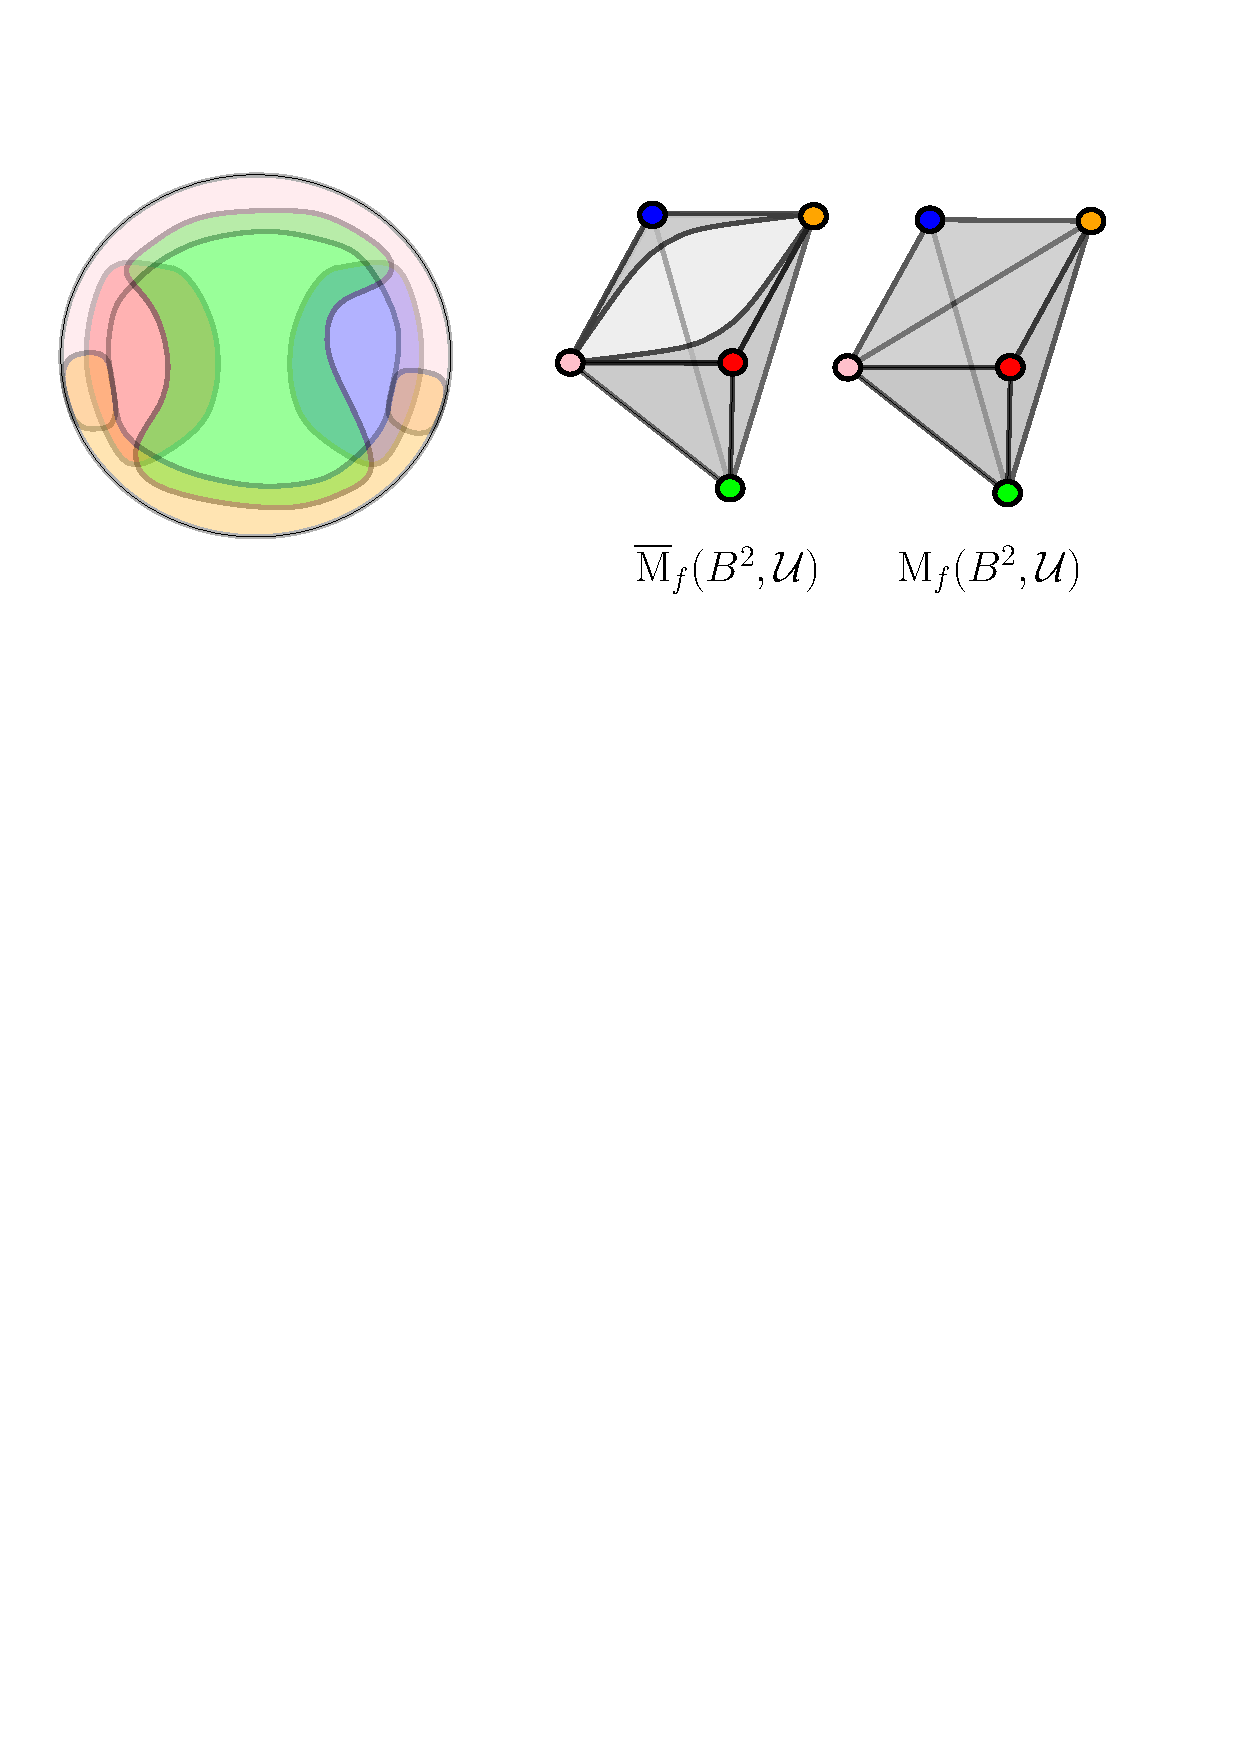
\includegraphics[height=5cm]{figures/CounterExampleHomoSurjection}
\caption[(MultiNerve) Mapper with bivariate map]{\label{fig:cover} The domain is the disk $B^2$, and we consider the identity function $f$,
as well as a generic open minimal cover $\U$ with five elements.
The MultiNerve Mapper is homeomorphic to the disk $B^2$ and the Mapper is homeomorphic to the sphere $\mathbb S^2$.
Then, $H_2(\Mapper_f(B^2,\U))\neq 0$ while $H_2(\MMapper_f(B^2,\U))=0$.}
\end{center}\end{figure}























%%%%%%%%%%%%%%%%%%%%%%%%%%%%%%%%%%%%%%%%%%%%%%%%%%%%%%%%%%%%%%%%%%%%%%%%%%%
\section{Structure of the MultiNerve Mapper}
\label{sec:structure}

In this section, we study and characterize the topological structure of the (MultiNerve) Mapper computed on a non discrete topological space.
More precisely, we show that this topological structure can be read off
from the extended persistence diagram of the Reeb graph. %in a way that depends only on the gomic. 
%specific zigzag persistence barcode, called the {\em cover zigzag persistence barcode}, that depends only on the gomic $\I$.
%$f^{\rm M}_{\I}$.
To prove this, we show that the MultiNerve Mapper $\MMapper_f(X,\I)$ is actually isomorphic (as a combinatorial multigraph)
to a specific Reeb graph, %$\Reeb_{\fMM}$, 
whose extended persistence diagram is related to 
the extended persistence diagram $\Dg(\tilde f)$ of $\Reeb_f(X)$. 

\paragraph*{Notation.} In the following, the combinatorial version of the Reeb graph (where each critical point is 
turned into a node and where the functional and metric information is forgotten) is
denoted by $\mathcal{C}\Reeb_f(X)$.

%However, this result is not completely satisfying regarding stability. Indeed, stability results 
%for zigzag persistence barcodes are, to our knowledge, only phrased with levelset zigzag persistence barcodes
%i.e. the upper bound is the interleaving distance between zigzag persistence modules
%~\cite{Botnan16}. Since we wish to state stability results in the same vein as Theorems~\ref{th:Stab} and~\ref{th:ExStab},
%we then relate this cover zigzag persistence barcode to the levelset zigzag persistence barcode of the Reeb graph---more precisely to its
%extended persistence diagram, which is equivalent according to Corollary~\ref{cor:EPZZ}. 
%(namely a simplification of the extended persistence diagram of the Reeb graph).
%This extended persistence diagram is finally used to prove
%a stability result with an extension of the bottleneck distance that only depends on the gomic $\I$. 
 
%This structure is described in Section~\ref{sec:topoMultiNerve}, and encoded in a signature in
%Section~\ref{sec:MultiNerveSign} for the MultiNerve Mapper and in Section~\ref{sec:MapperSign}
%for the Mapper.

\subsection{Topological structure of the MultiNerve Mapper}
\label{sec:topoMultiNerve}

%In this section, we show that a specific zigzag persistence barcode, called the {\em cover zigzag persistence barcode},
%encodes the topological structure of the MultiNerve Mapper. %that depends only on the gomic $\I$.

%We recall that this topological structure is already encoded in the extended persistence diagram of $f_{\I}$,
%thanks to the bag-of-feature interpretation of extended persistence diagrams for graphs.
%However, this alternative way of encoding the topological structure of the MultiNerve Mapper avoids
%the choice of an arbitrary function $f_{\I}$, and is more easily relatable to the Reeb graph. 
%avoid chosing an arbitrary function $f_{\I}$ as in Definition~\ref{def:arbitfunc}.

In order to show that the MultiNerve Mapper is a specific Reeb graph, 
we first show that (MultiNerve) Mappers can be equipped with functions. %$\fMM$, and that,
%as a multigraph, it is isomorphic to its Reeb graph.  

\begin{defin}\label{def:arbitfunc}
Let $\I=\{I_\alpha\}_{\alpha\in A}$ be a gomic of $\im(f)$ and 
$\V=\{V^i_\alpha\}_{\substack{1\leq i \leq c(\alpha), \alpha\in A}}$ be the associated
connected pullback cover. 
Then we define $\fMM:\MMapper_f(X,\I)\rightarrow\R$ 
as the piecewise-linear extension of the function defined
on the nodes of $\MMapper_f(X,\I)$ by
$V_\alpha^i\mapsto{\rm mid}(\tilde I_\alpha)$,
where ${\rm mid}(\tilde I_\alpha)$ is the midpoint of the proper subinterval $\tilde I_\alpha$ of $I_\alpha$.
The definition of $\fM:\Mapper_f(X,\I)\rightarrow\R$ is similar. 
\end{defin}

Hence, Reeb graphs can be computed from $\MMapper_f(X,\I)$ and $\Mapper_f(X,\I)$, once they are equipped with $\fMM$ and $\fM$ respectively.
Let us call them $\Reeb_{\fMM}(\MMapper_f(X,\I))$ and $\Reeb_{\fM}(\Mapper_f(X,\I))$,
with corresponding induced maps 
${\fMMR}:\Reeb_{\fMM}(\MMapper_f(X,\I))\rightarrow\R$ and $\fMR:\Reeb_{\fM}(\Mapper_f(X,\I))\rightarrow\R$.
The following lemma, which states that (MultiNerve) Mappers are isomorphic to their Reeb graphs, is a simple consequence of Remark~\ref{rem:idemreeb}.

\begin{lem}\label{lem:idemMapper}
Let $X$ be a topological space and $f:X\rightarrow\R$ be a Morse-type function.
Let $\I$ be a gomic of $\im(f)$.
Then $\MMapper_f(X,\I)$ and $\mathcal C\Reeb_{\fMM}(\MMapper_f(X,\I))$ are isomorphic as combinatorial multigraphs.
The same is true for $\Mapper_f(X,\I)$ and $\mathcal C\Reeb_{\fM}(\Mapper_f(X,\I))$.
\end{lem}  

%is a simplification of the one of the Reeb graph.
%In order to do this, we need to relate the levelset zigzag persistence barcode of a MultiNerve Mapper to the associated gomic. 
%This is done using {\em cover zigzag modules}.

Hence, by a slight abuse of notation, we rename $\tilde{\sf m}_{\I}$ %:\Reeb_{\fM}(\Mapper_f(X,\I))\rightarrow\R$ 
and  $\tilde{\bar{\sf m}}_{\I}$ %:\Reeb_{\fMM}(\MMapper_f(X,\I))\rightarrow\R$ 
into $\fM$ and $\fMM$ for convenience. 

We now state the main result of this section, which ensures that the extended persistence diagram $\Dg(\fMM)$, i.e. the bag-of-features signature of 
$\Reeb_{\fMM}(\MMapper_f(X,\I))$ and $\MMapper_f(X,\I)$,  
is nothing but a simplification of  $\Dg(\tilde f)$, i.e. the bag-of-features signature of $\Reeb_{f}(X)$.

\begin{thm}
\label{th:ExDgMultiNerve}
Let $X$ be a topological space and $f:X\rightarrow\R$ be a Morse-type function. Let $\Reeb_f(X)$ be the corresponding Reeb graph
and $\tilde f : \Reeb_f(X)\rightarrow\R$ be the induced map.
Let $\I$ be a gomic of ${\rm im}(f)$. %, and let $f_{\I}:\MMapper_f(X,\I)\rightarrow\R$. 
There are bijections between:

\begin{center}
\begin{tabular}{ll}
{\rm (i)} %{\rm I}-$\CZZ_0(f,\I)$ 
$\Ord_0(\fMM)$ 
and $\Ord_0(\tilde f)\setminus Q_O^{\I}$ & 
{\rm (iii)} %{\rm IV}-$\CZZ_0(f,\I)$ 
$\Ext_1^-(\fMM)$ 
and $\Ext_1^-(\tilde f)\setminus Q_{E^-}^{\I}$\\[0.5em]
{\rm (ii)} %{\rm II}-$\CZZ_0(f,\I)$ 
$\Rel_1(\fMM)$ 
and $\Rel_1(\tilde f)\setminus Q_R^{\I}$ &
{\rm (iv)} %{\rm III}-$\CZZ_0(f,\I)$ 
$\Ext_0^+(\fMM)$ 
and $\Ext_0^+(\tilde f)$
\end{tabular}
\end{center}
where $\StairOrd=\bigcup_{I\in\I}Q_{{\tilde I}\cup I_\cap^+}^+$,
$\StairRel=\bigcup_{I\in\I}Q_{{\tilde I}\cup I_\cap^-}^-$, and
$\StairExtMM=\bigcup_{I\in\I}Q_I^-$, and where, for any interval $I$ with endpoints $a\leq b$, we let
$Q_I^+ =\{(x,y)\in\R^2\,:\, a\leq x\leq y\leq b\}$ be the corresponding half-square
above the diagonal, and $Q_I^- =\{(x,y)\in\R^2\,:\, a\leq y< x\leq
b\}$ be  the half-square strictly below the diagonal. See Figure~\ref{fig:staircase} for an illustration.
\end{thm}

%%%
\begin{figure}[h]\centering
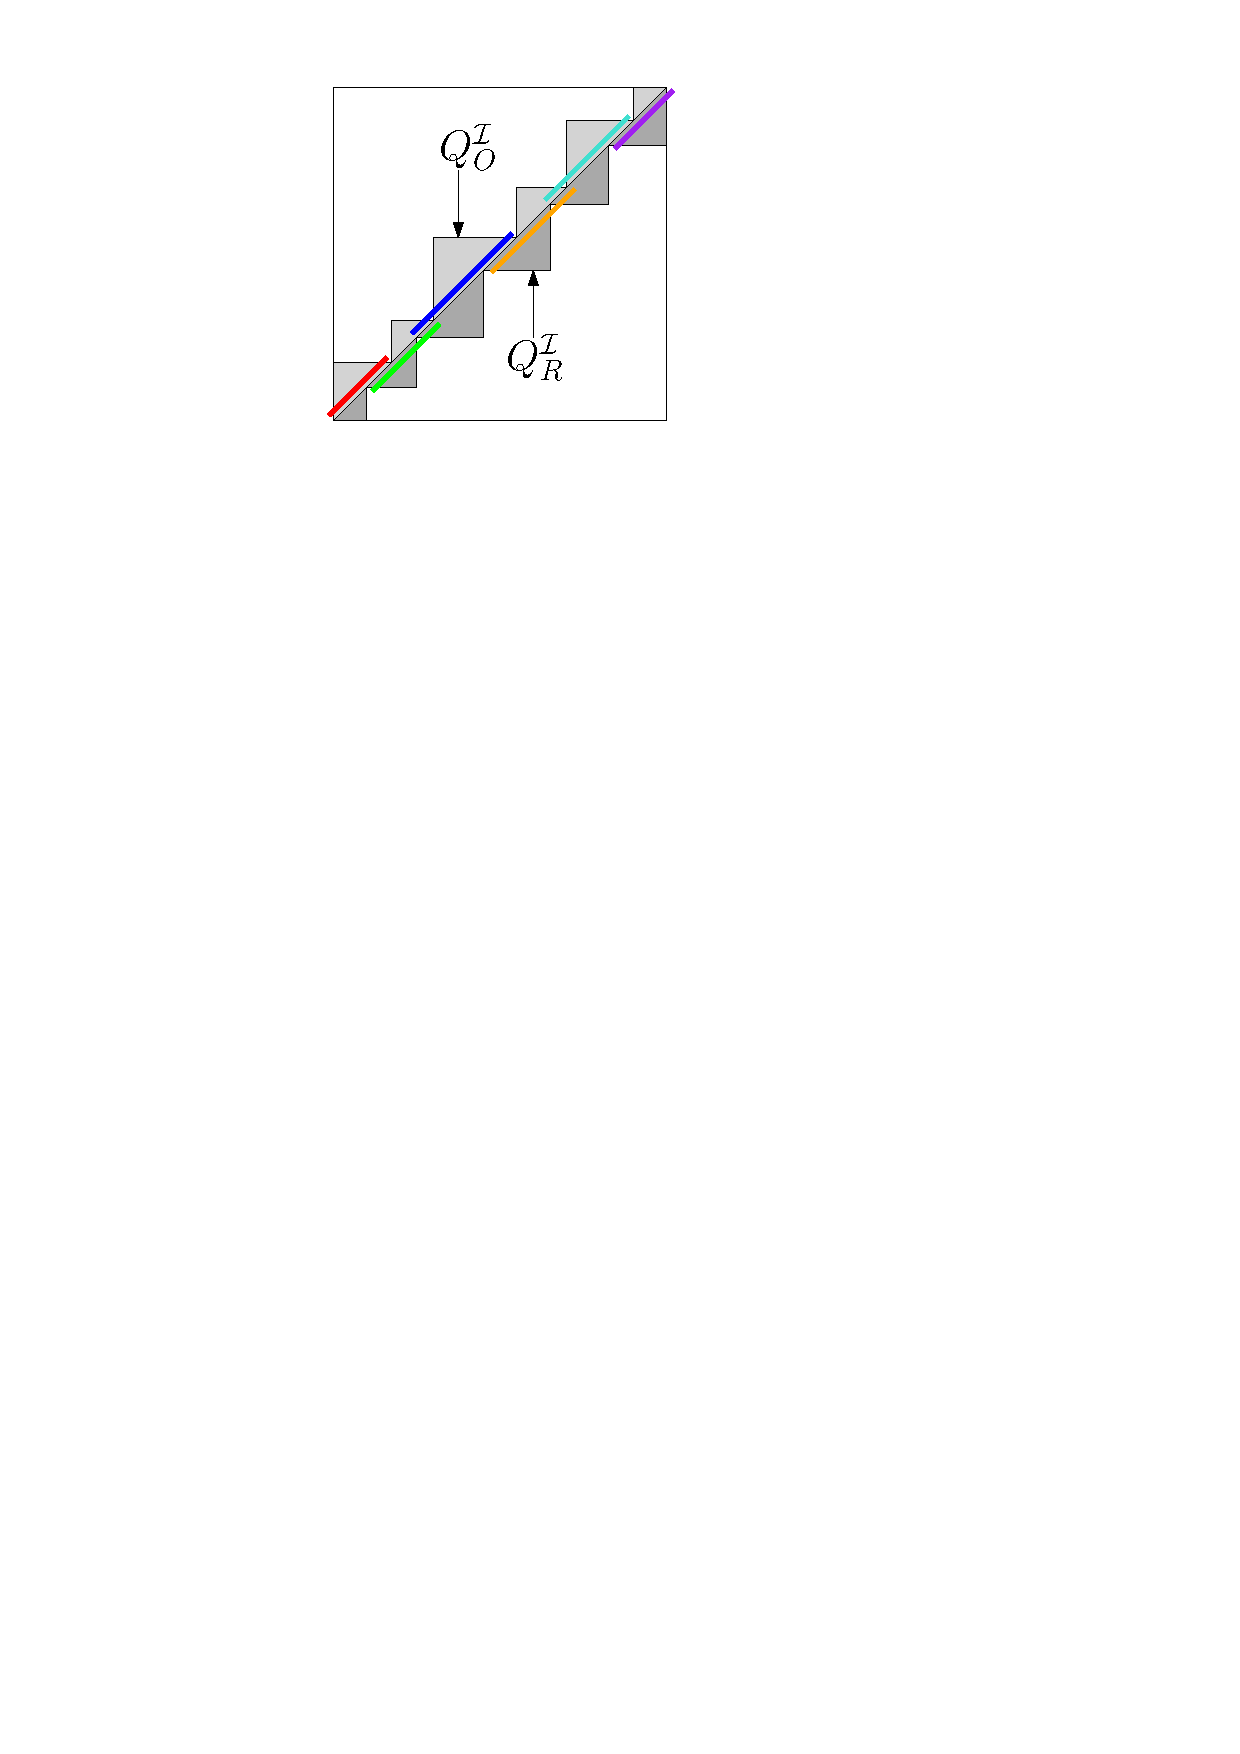
\includegraphics[height = 4cm]{figures/StaircaseOrdRel}\ \ \ \ 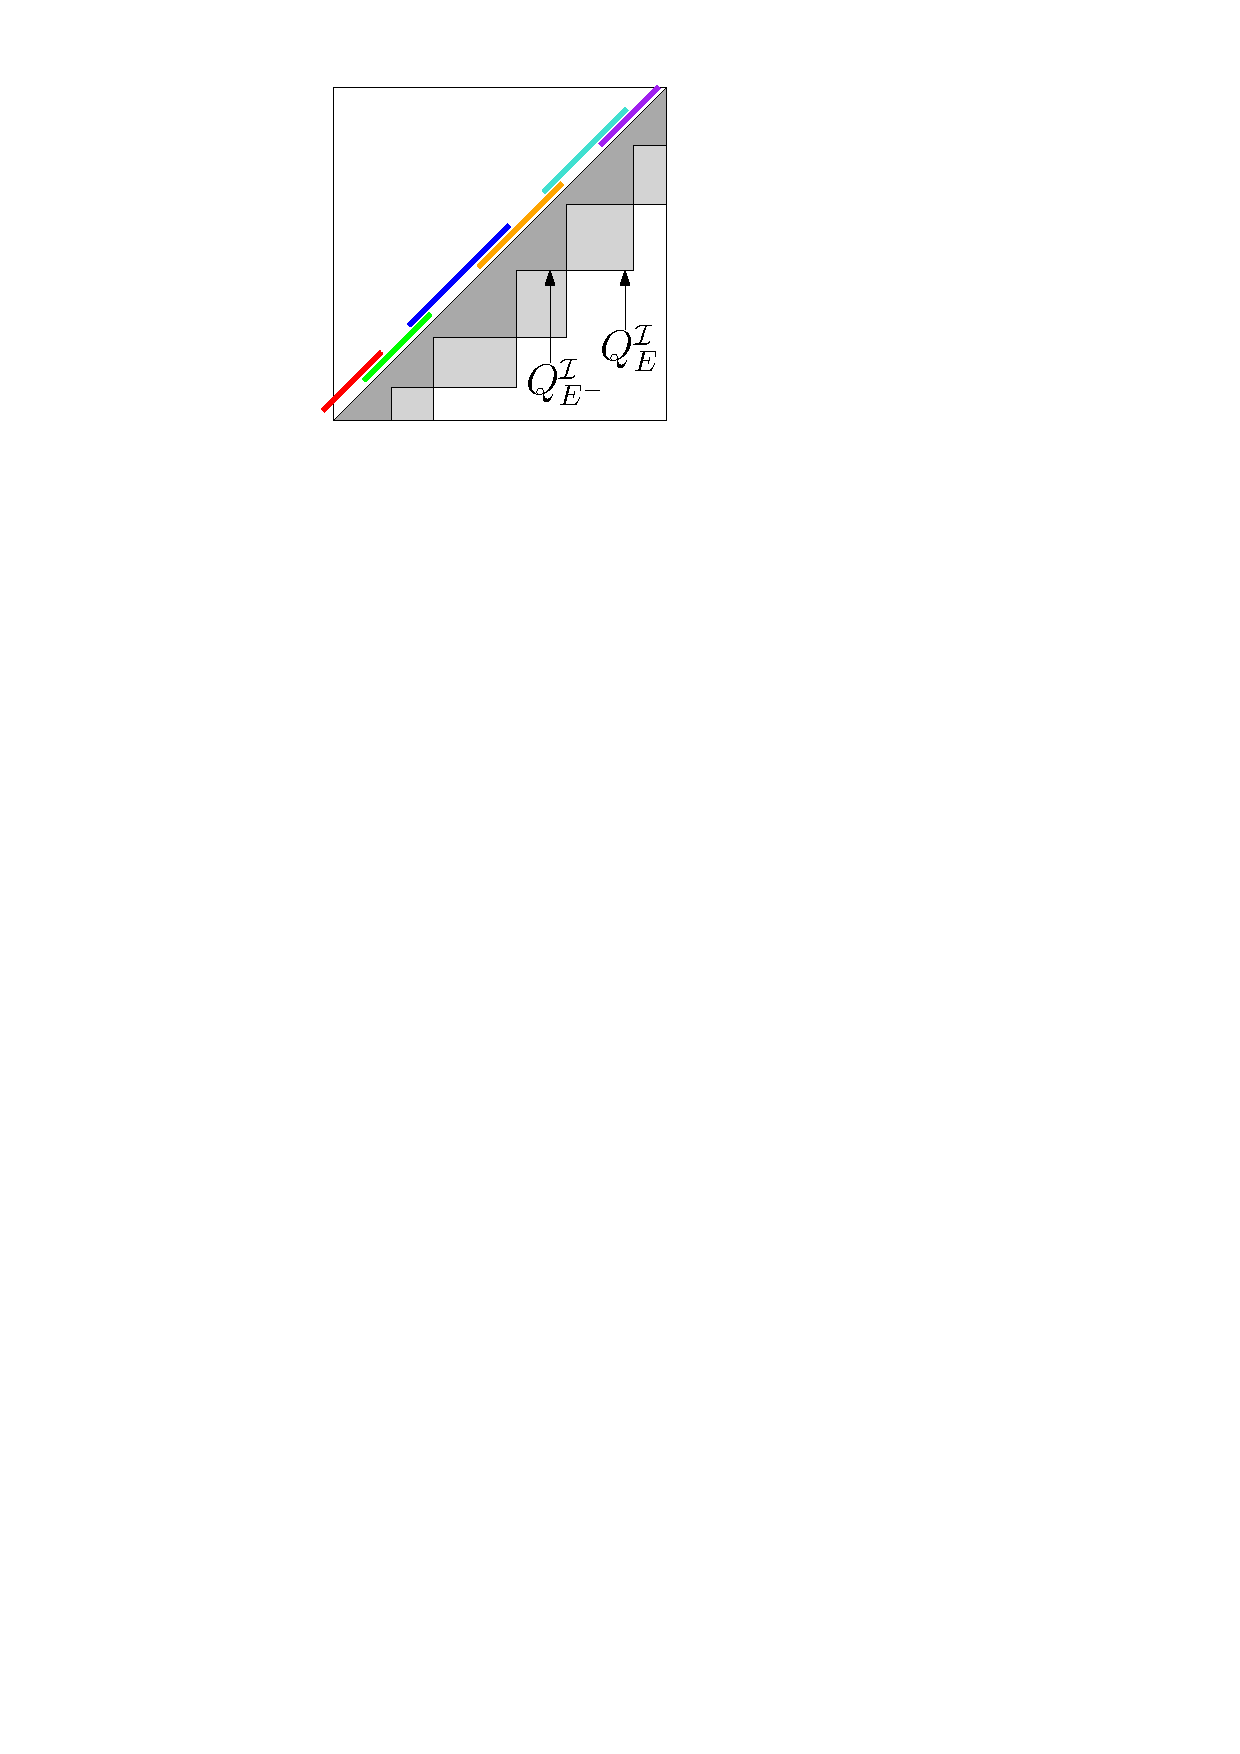
\includegraphics[height = 4cm]{figures/StaircaseExt}
\caption{Left: Staircases of ordinary (light grey) 
and relative (dark grey) types.
Right: Staircases of extended types---$Q_{E^-}^{\I}$ is in dark grey while $Q_{E}^{\I}$ 
is the union of $Q_{E^-}^{\I}$ with the light grey area.}
\label{fig:staircase}
\end{figure}

The remaining of Section~\ref{sec:topoMultiNerve} is devoted to the proof of Theorem~\ref{th:ExDgMultiNerve}.
In order to state the proof, we first introduce {\em cover zigzag persistence modules}. 

\begin{defin}\label{def:coverZZ}
Let $X$ be a topological space and $f:X\rightarrow\R$ be a Morse-type function.
Let $\I=\{I_\alpha\}_{1\leq\alpha\leq m}$ be a gomic of $\im(f)$, sorted by the natural order defined in Section~\ref{sec:1Dmapper}. 
%$I_\alpha\cap I_\beta\neq \emptyset$ only if $|\beta-\alpha|\leq 1$. %in the total order yielded be Lemma~\ref{lem:minimal-cover_1-dim}.

Let $\Crit(f)=\{-\infty=a_0,a_1,...,a_n,a_{n+1}=+\infty\}$. 
%and $\LZZ(f)=H_*\left(X_0^0\hookrightarrow X_0^1\hookleftarrow X_1^1\hookrightarrow 
%X_1^2\hookleftarrow\cdots\hookrightarrow X_{n-1}^n\hookleftarrow X_n^n\right)$.
%where $H_*$ is the homology functor.
For any open interval $I$ with left endpoint $a$, 
we define the integers $l(I)$, $r(I)$ by $l(I)=\max\{i\,:\,a_i\leq a\}$
and $r(I)=\max\{l(I),\max\{i\,:\,a_i\in I\}\}$.
Then, we define the {\em cover zigzag persistence module} $\CZZ(f,\I)$ by 
$$\CZZ(f,\I)=H_*\left(X_{l(I_1)}^{r(I_1)}\hookleftarrow X_{l(I_1\cap I_2)}^{r(I_1\cap I_2)}\hookrightarrow X_{l(I_2)}^{r(I_2)}\hookleftarrow X_{l(I_2\cap I_3)}^{r(I_2\cap I_3)}
\hookrightarrow \cdots \hookleftarrow X_{l(I_{m-1}\cap I_m)}^{r(I_{m-1}\cap I_m)}\hookrightarrow X_{l(I_m)}^{r(I_m)}\right),$$
where the $X_i^j$ spaces are as in Definition~\ref{def:LZZ}.
We also let $\DgCZZ(f,\I)$ denote the barcode of this module.
\end{defin}


Note that cover zigzag persistence modules can be isometrically embedded (with the bottleneck and Wasserstein distances) 
into the south face of the Mayer-Vietoris half-pyramid. Indeed, each node of $\CZZ(f,\I)$ belongs to this south face.
The only difficulty is that $\CZZ(f,\I)$ may include the same node several times consecutively when there is a sequence of 
consecutive intervals in the gomic that are all included between two consecutive critical values of $f$, i.e. for which $l(I)=r(I)$. 
However, in that case, the corresponding arrows in the module are isomorphisms.
Thus, composing these arrows leaves the resulting barcode unchanged.  

%We now show that this barcode is indeed a complete descriptor---see also Lemma~2 in~\cite{Babu13}: 
%The cover zigzag module of a space encodes the same topological information as the MultiNerve Mapper computed with the same
%gomic, as stated in the following lemma

\begin{lem}\label{lem:CoverZZ}
Let $X$ be a topological space and $f:X\rightarrow\R$ be a Morse-type function.
Let $\I$ %=\{I_\alpha\}_{1\leq\alpha\leq m}$ 
be a gomic of ${\rm im}(f)$. %and let $f_{\I}:\MMapper_f(X,\I)\rightarrow\R$ be as in Definition~\ref{def:arbitfunc}. 
Then, there is a bijection between $\Dg(\fMM)$ and $\DgCZZ_0(f,\I)$. 
%$$\DgZZ_0(f_{\I})\simeq\DgCZZ_0(f,\I).$$
%$\DgCZZ_0(f,\I)$ is a bag-of-feature descriptor of the topological structure of $\MMapper_f(X,\I)$.
\end{lem}

\begin{proof}
%Since extended persistence diagrams are already bag-of-feature descriptors, all we have to show is that there is
%a bijection between intervals of $\DgCZZ_0(f,\I)$ and points of $\Dg(g)$, where $g:\MMapper_f(X,\I)\rightarrow\R$
%is the piecewise-linear extension on edges of an arbitrary monotonic function defined on the nodes of $\MMapper_f(X,\I)$,
%with the order on nodes being induced by the order on gomic elements. Moreover, there is 
%a bijection between $\Dg(g)$ and $\DgZZ_0(g)$ according to Corollary~\ref{cor:EPZZ}, so we only have to relate $\DgCZZ_0(f,\I)$
%to the levelset zigzag persistence barcode $\DgZZ_0(g)$. 

Recall from Corollary~\ref{cor:EPZZ} that it suffices to show that 
$\LZZ_0(\fMM)$ and $\CZZ_0(f,\I)$ are isomorphic as zigzag persistence modules. 
Assume without loss of generality that $\I$ has $m$ elements, with $m\in\N^*$.
%We have to show that $\LZZ(f_{\I})$ and $\CZZ(f,\I)$ are isomorphic in dimension 0. 
First, note 
%recall from Definition~\ref{def:arbitfunc} 
that $\card(\Crit(\fMM))$ is equal to $m$. Hence, both $\LZZ(\fMM)$ and $\CZZ(f,\I)$ have exactly $2m+1$ nodes.
Moreover, since the MultiNerve Mapper tracks the connected components of the interval and intersection preimages of $f$,
each element of $\LZZ_0(\fMM)$ is of the form $H_0(f^{-1}(I))$, $I\in\I$, or $H_0(f^{-1}(I\cap J))$, $I,J$ consecutive in $\I$.

Let $I\in\I$.
Since $f$ is Morse-type, $X_{l(I)}^{r(I)}$ and $X^I=f^{-1}(I)$ have the same 
homotopy type. Indeed, recall from Definition~\ref{def:LZZ} that there exist $s_{l(I)}$ and $s_{r(I)}$ such that 
$X_{l(I)}^{r(I)}=f^{-1}\left(\left[s_{l(I)},s_{r(I)}\right]\right)$ 
and $s_{l(I)}$ (resp. $s_{r(I)}$) and the left (resp. right) endpoint of $I$
are located between the same consecutive critical values of $f$.  
In particular, $X_{l(I)}^{r(I)}$ and $X^I$ have the same number of connected components, meaning that 
$H_0(X^I)$ and $H_0(X_{l(I)}^{r(I)})$ are isomorphic groups.
The same is also true for any $I\cap J$, $I,J\in\I$.

Hence, we define a canonical pointwise isomorphism $\Psi$ in dimension 0 as follows:
for each node, %of $\LZZ_0(g)$ %, which is of the form $H_0(f^{-1}(I))$ or $H_0(f^{-1}(I\cap J))$, 
send each connected component of one preimage, or equivalently each generator of one homology group, 
to the connected component of the other preimage which intersects it 
(there is only one since the preimages have the same number of connected components). %connected component of between the modules.
By definition of the MultiNerve Mapper, $\Psi$ commutes with the canonical inclusion.
Hence, $\LZZ_0(\fMM)$ and $\CZZ_0(f,\I)$ are isomorphic. %in dimension 0.
\end{proof}













Finally, we  relate the cover zigzag persistence barcode to the extended persistence diagram of the Reeb graph.
Namely, we show that a specific simplification of this extended persistence diagram encodes the same information as the 
cover zigzag persistence barcode. %(Theorem~\ref{th:ExDgMultiNerve}). 
%Hence, since stability results are already available for extended persistence diagrams and can be easily adapted,
%we use this simplified diagram as a signature for the MultiNerve Mapper.

%Lemma~\ref{lem:CoverZZ}, together with Corollary~\ref{cor:EPZZ}, allows us to prove Theorem~\ref{th:ExDgMultiNerve} below,
%which describes the topological structure of the MultiNerve Mapper directly from
%the gomic $\I$ and the extended persistence diagram of $\tilde f$. There is a similar statement 
%with zigzag persistence barcodes, but we only phrase it with extended persistence since
%we use extended persistence extensively in the other chapters of this thesis. 
%We provide one more definition in order to state the simplification we use. %before stating Theorem~\ref{th:ExDgMultiNerve}.

%\begin{defin}
%Given an interval
%$I=(a,b)$ (indifferently open, closed or half-open), let
%$Q_I^+ =\{(x,y)\in\R^2\,:\, a\leq x\leq y\leq b\}$ be the half-square
%above the diagonal, and $Q_I^- =\{(x,y)\in\R^2\,:\, a\leq y< x\leq
%b\}$ the half-square strictly below the diagonal.
%
%Now, let $\I$ be a gomic. Decompose each interval $I\in \I$ as
%$I=I_\cap^-\sqcup {\tilde I}\sqcup I_\cap^+\in\I$,
%then let $\StairOrd=\bigcup_{I\in\I}Q_{{\tilde I}\cup I_\cap^+}^+$,
%$\StairRel=\bigcup_{I\in\I}Q_{{\tilde I}\cup I_\cap^-}^-$, and
%$\StairExtMM=\bigcup_{I\in\I}Q_I^-$. %and $\StairExtM=\bigcup_{\substack{I,J\in\I \\ I\cap J\neq\emptyset}}Q_{I\cup J}^-$.
%\end{defin}

%See Figure~\ref{fig:staircase} for an illustration. These staircases outline the areas of the plane that cover features that disappear when
%computing the MultiNerve Mapper, as stated in Theorem~\ref{th:ExDgMultiNerve} below.
%%%%
%\begin{figure}[h] \begin{center}
%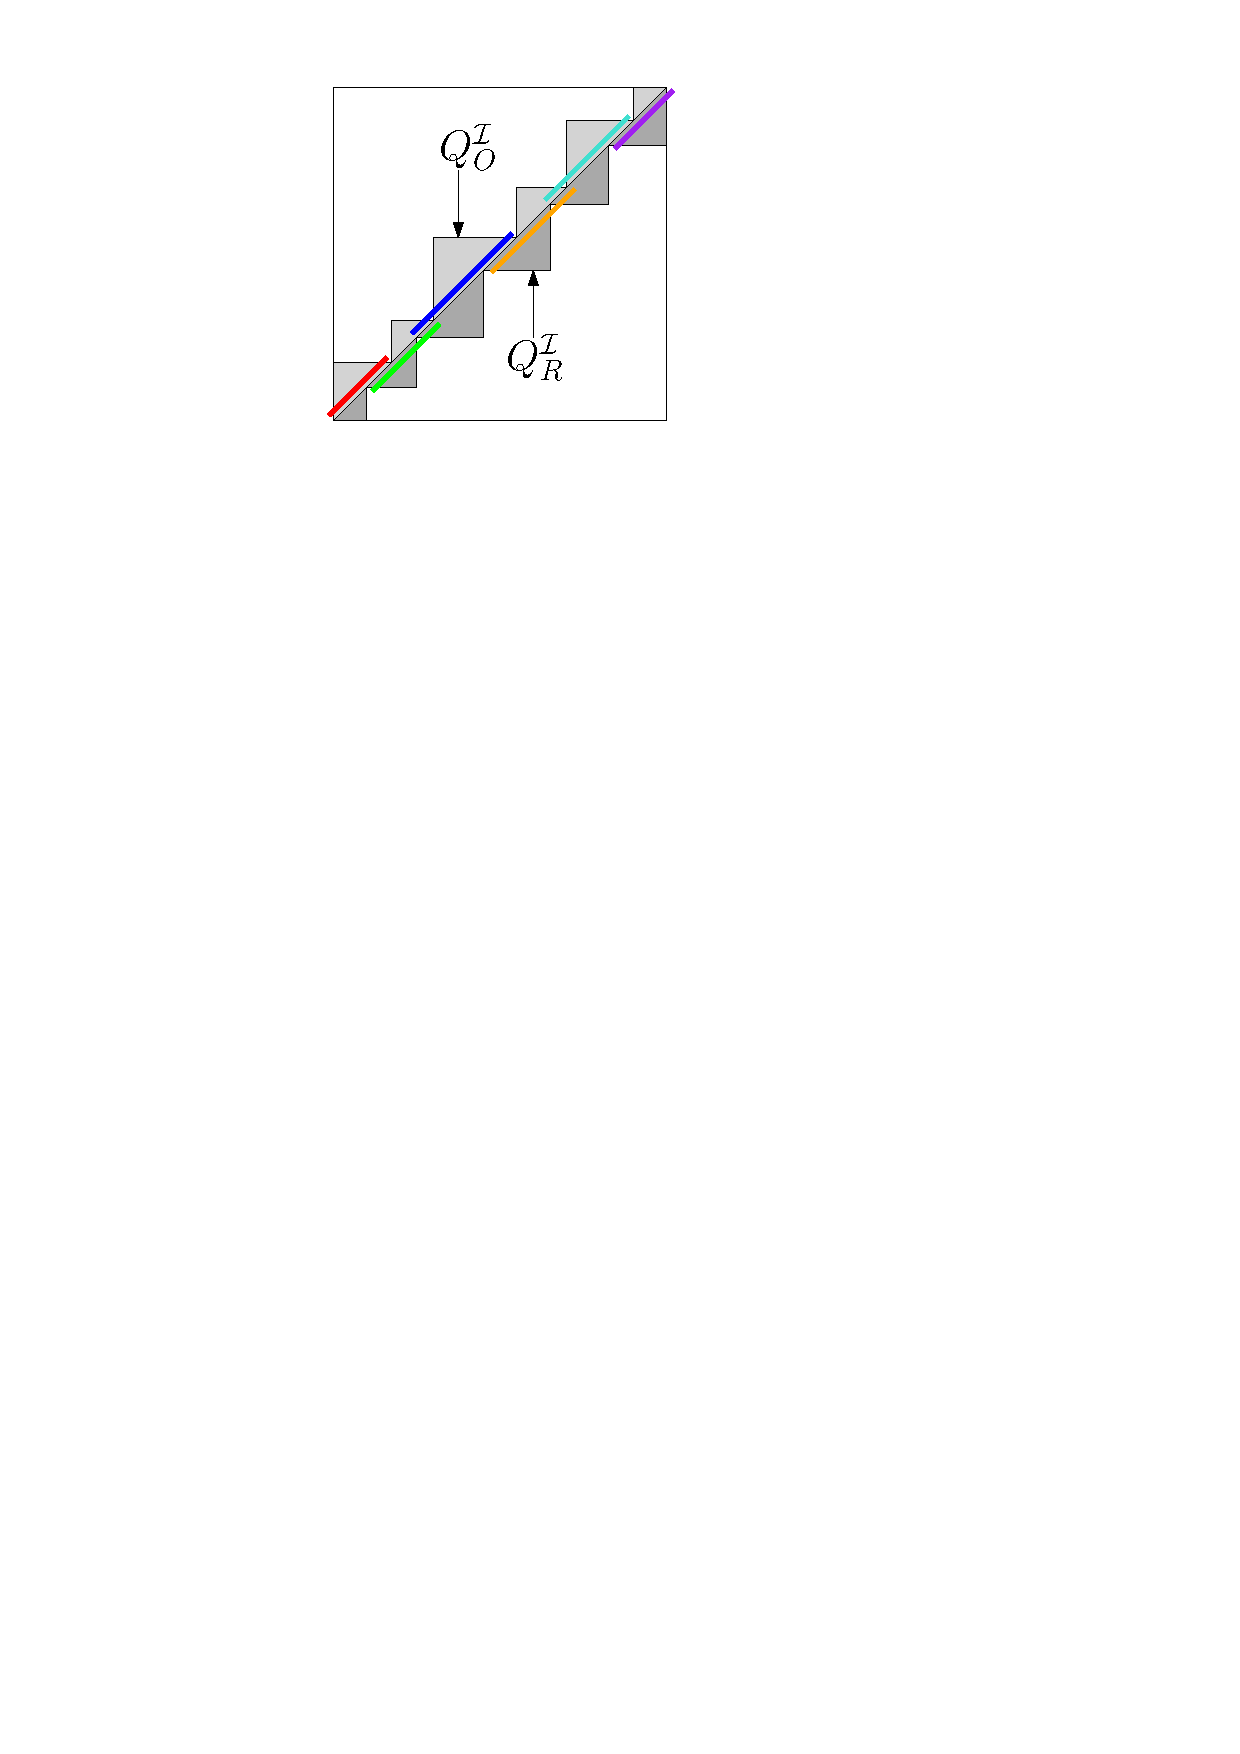
\includegraphics[height = 4cm]{figures/StaircaseOrdRel}\hspace{3mm}\ \ \ \ 
%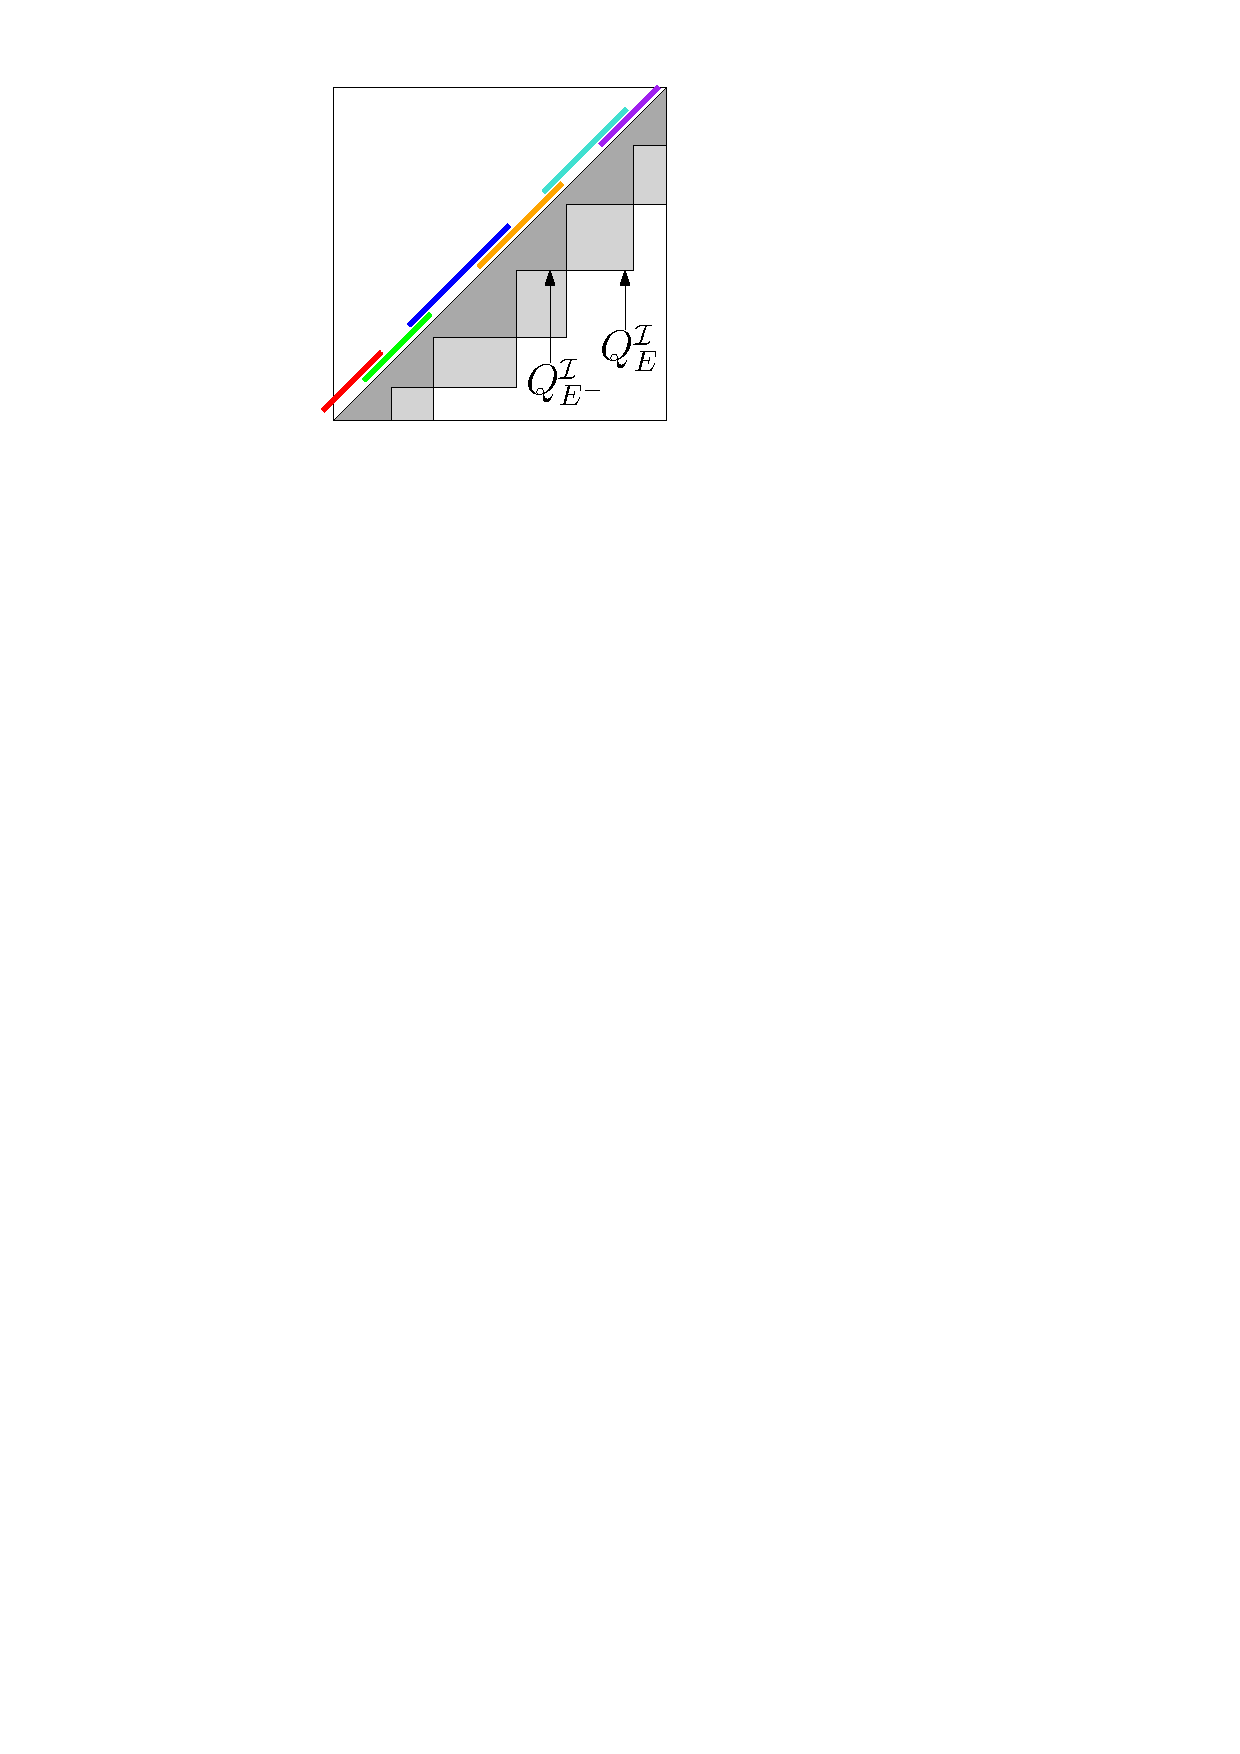
\includegraphics[height = 4cm]{figures/StaircaseExt}\hspace{3mm}
%\caption[Staircases]{\label{fig:staircase} Left: Staircases of ordinary (light grey) 
%and relative (dark grey) types.
%Right: Staircases of extended types---$Q_{E^-}^{\I}$ is in dark grey while $Q_{E}^{\I}$ 
%is the union of $Q_{E^-}^{\I}$ with the light grey area.}
%\end{center} \end{figure}



%\begin{thm}
%\label{th:ExDgMultiNerve}
%Let $X$ be a topological space and $f:X\rightarrow\R$ be a Morse-type function. Let $\Reeb_f(X)$ be the corresponding Reeb graph
%and $\tilde f : \Reeb_f(X)\rightarrow\R$ be the induced map.
%Let $\I$ be a gomic of ${\rm im}(f)$. %, and let $f_{\I}:\MMapper_f(X,\I)\rightarrow\R$. 
%There are bijections between:
%\begin{center}
%\begin{tabular}{ll}
%{\rm (i)} %{\rm I}-$\CZZ_0(f,\I)$ 
%$\Ord_0(\fMM)$ 
%and $\Ord_0(\tilde f)\setminus Q_O^{\I}$ & 
%{\rm (iii)} %{\rm IV}-$\CZZ_0(f,\I)$ 
%$\Ext_1^-(\fMM)$ 
%and $\Ext_1^-(\tilde f)\setminus Q_{E^-}^{\I}$\\[0.5em]
%{\rm (ii)} %{\rm II}-$\CZZ_0(f,\I)$ 
%$\Rel_1(\fMM)$ 
%and $\Rel_1(\tilde f)\setminus Q_R^{\I}$ &
%{\rm (iv)} %{\rm III}-$\CZZ_0(f,\I)$ 
%$\Ext_0^+(\fMM)$ 
%and $\Ext_0^+(\tilde f)$
%\end{tabular}
%\end{center}
%\end{thm}

\begin{proof}[Proof of Theorem~\ref{th:ExDgMultiNerve}]
Again, recall from Corollary~\ref{cor:EPZZ} 
that $\Dg(\tilde f)$ encodes the same information as $\DgZZ_0(\tilde f)$. Hence, since $\Dg(\fMM)$ and $\DgCZZ_0(f,\I)$ are equivalent
from Lemma~\ref{lem:CoverZZ}, we focus on the relation between
$\DgZZ_0(\tilde f)$ and $\DgCZZ_0(f,\I)$.
As mentioned after Definition~\ref{def:coverZZ},
the cover zigzag persistence module $\CZZ(f,\I)$ can be isometrically embedded in the south face of the Mayer-Vietoris half-pyramid.
Hence, we can assume without loss of generality that the set of nodes of $\CZZ(f,\I)$
is a subset of the nodes of a monotone zigzag module $\overline\CZZ(f,\I)$ %with 0-dimensional barcode $\overline\DgCZZ_0(f,\I)$ and
that can be drawn along the south face of the Mayer-Vietoris half-pyramid
by interpolating the elements of $\CZZ(f,\I)$.
Thus, it suffices by Theorem~\ref{th:MY} to study which intervals disappear when going from $\DgZZ_0(\tilde f)$ to $\overline\DgCZZ_0(f,\I)$ and then to $\DgCZZ_0(f,\I)$ 
using the pyramid rules recalled in Figure~\ref{fig:shiftZZ}.

\begin{figure}[h]\centering
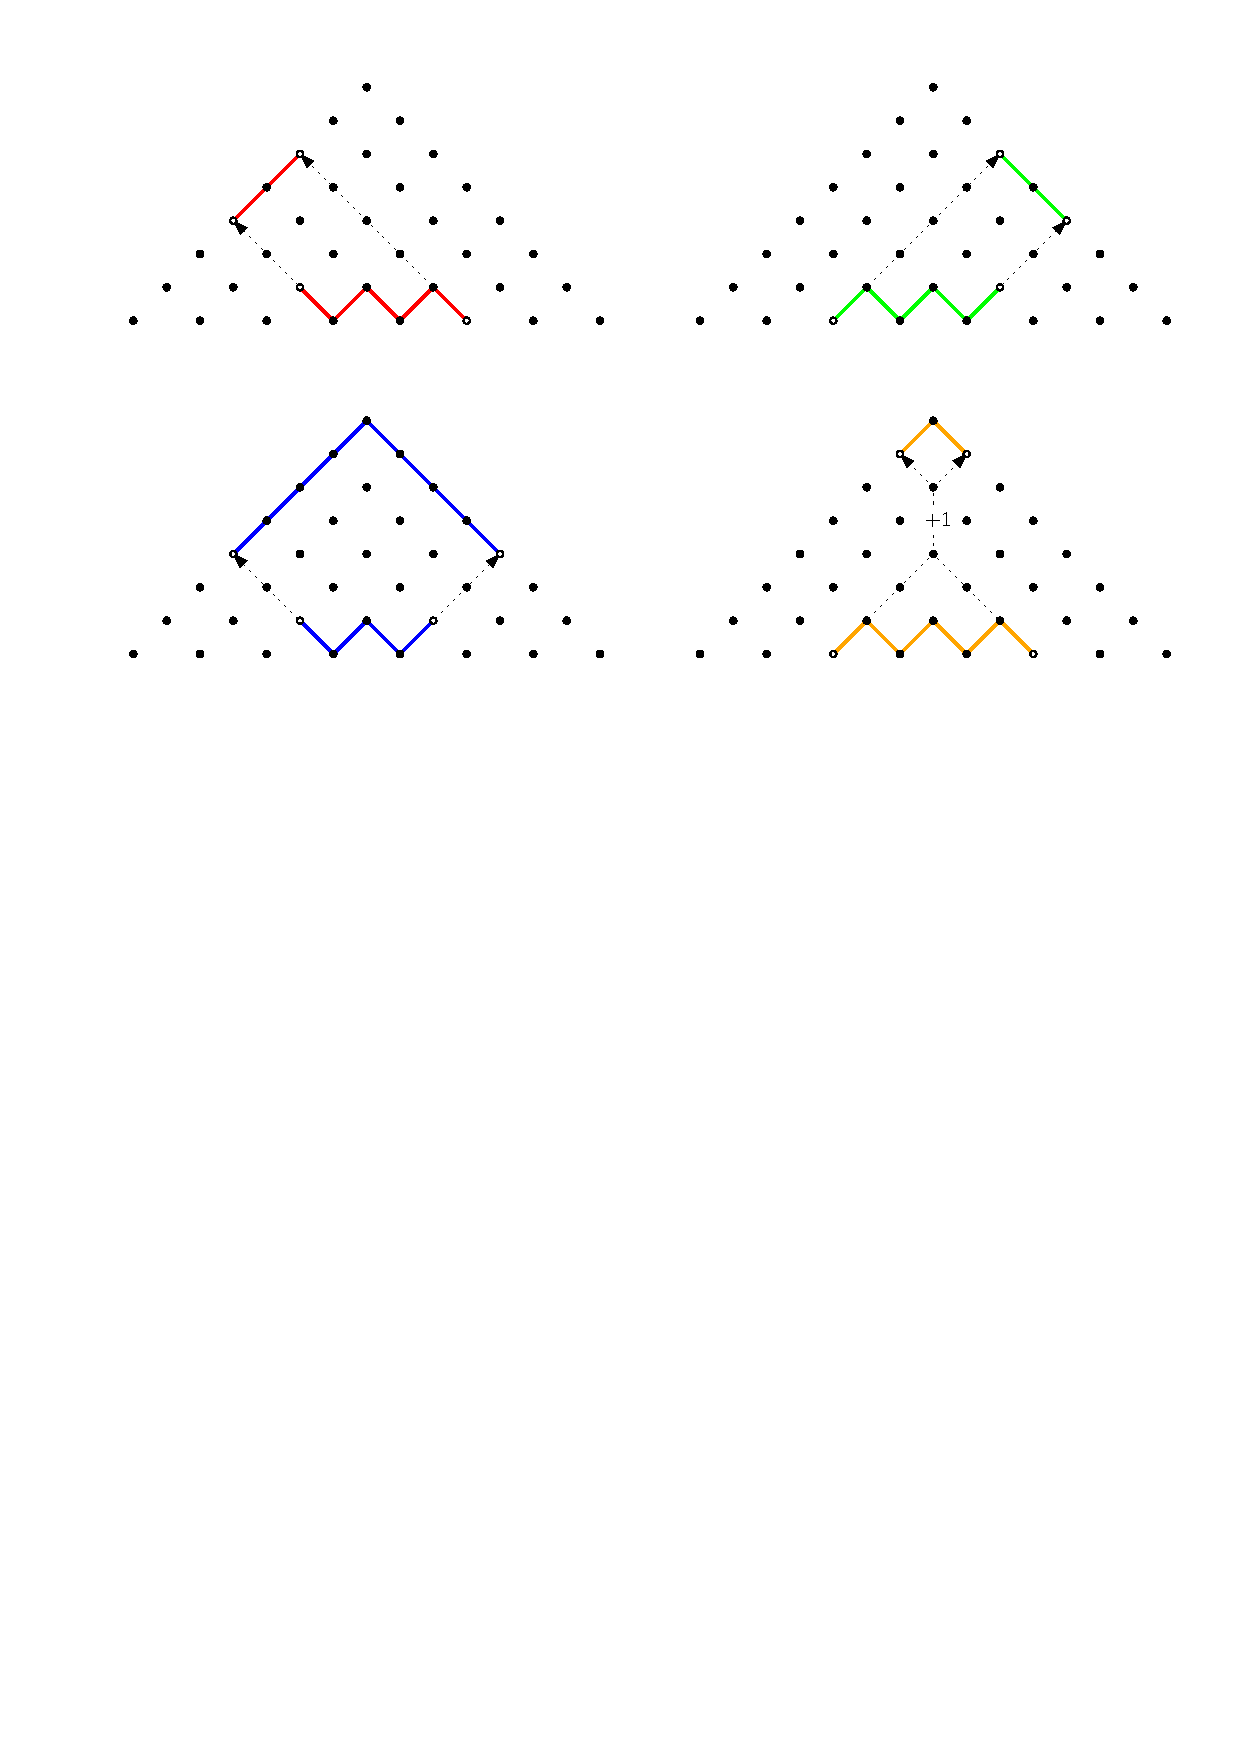
\includegraphics[width=15cm]{figures/ZZShift}
\caption[Pyramid rules]{\label{fig:shiftZZ} (From~\cite{Carlsson09b}) We show the
  axis of travel of birth and death endpoints of intervals of
  $\LZZ(f)$ to the up-down zigzag persistence module bounding the south face of
  the Mayer-Vietoris half-pyramid for interval modules that correspond
  to type I intervals (upper-left, red), type II intervals
  (upper-right, green), type III intervals (down-left, blue), and type IV
  intervals (down-right, orange) in $\DgZZ(f)$. The +1 in the
  down-right figure means that the homological dimension is increased
  by one.}
\end{figure}

We first give analogues of staircases for zigzag persistence. For any $I=I_\cap^-\sqcup \tilde I \sqcup I_\cap^+\in\I$, we define:
\begin{itemize}
\item ${\rm supp}_O(I)$ as the set of nodes of $\LZZ(f)$ that are located strictly between 
$X_{l(\tilde I\cup I_\cap^+)}^{l(\tilde I\cup I_\cap^+)}$ and $X_{r(\tilde I\cup I_\cap^+)-1}^{r(\tilde I\cup I_\cap^+)}$,
\item ${\rm supp}_R(I)$ as the set of nodes of $\LZZ(f)$ that are located strictly between 
$X_{l(I_\cap^-\cup \tilde I)}^{l(I_\cap^-\cup \tilde I)+1}$ and $X_{r(I_\cap^-\cup \tilde I)}^{r(I_\cap^-\cup \tilde I)}$, 
\item ${\rm supp}_{E^-}(I)$ as the set of nodes of $\LZZ(f)$ that are located strictly between $X_{l(I)}^{l(I)+1}$ and $X_{r(I)-1}^{r(I)}$. 
\end{itemize}



\begin{figure}[h]\centering
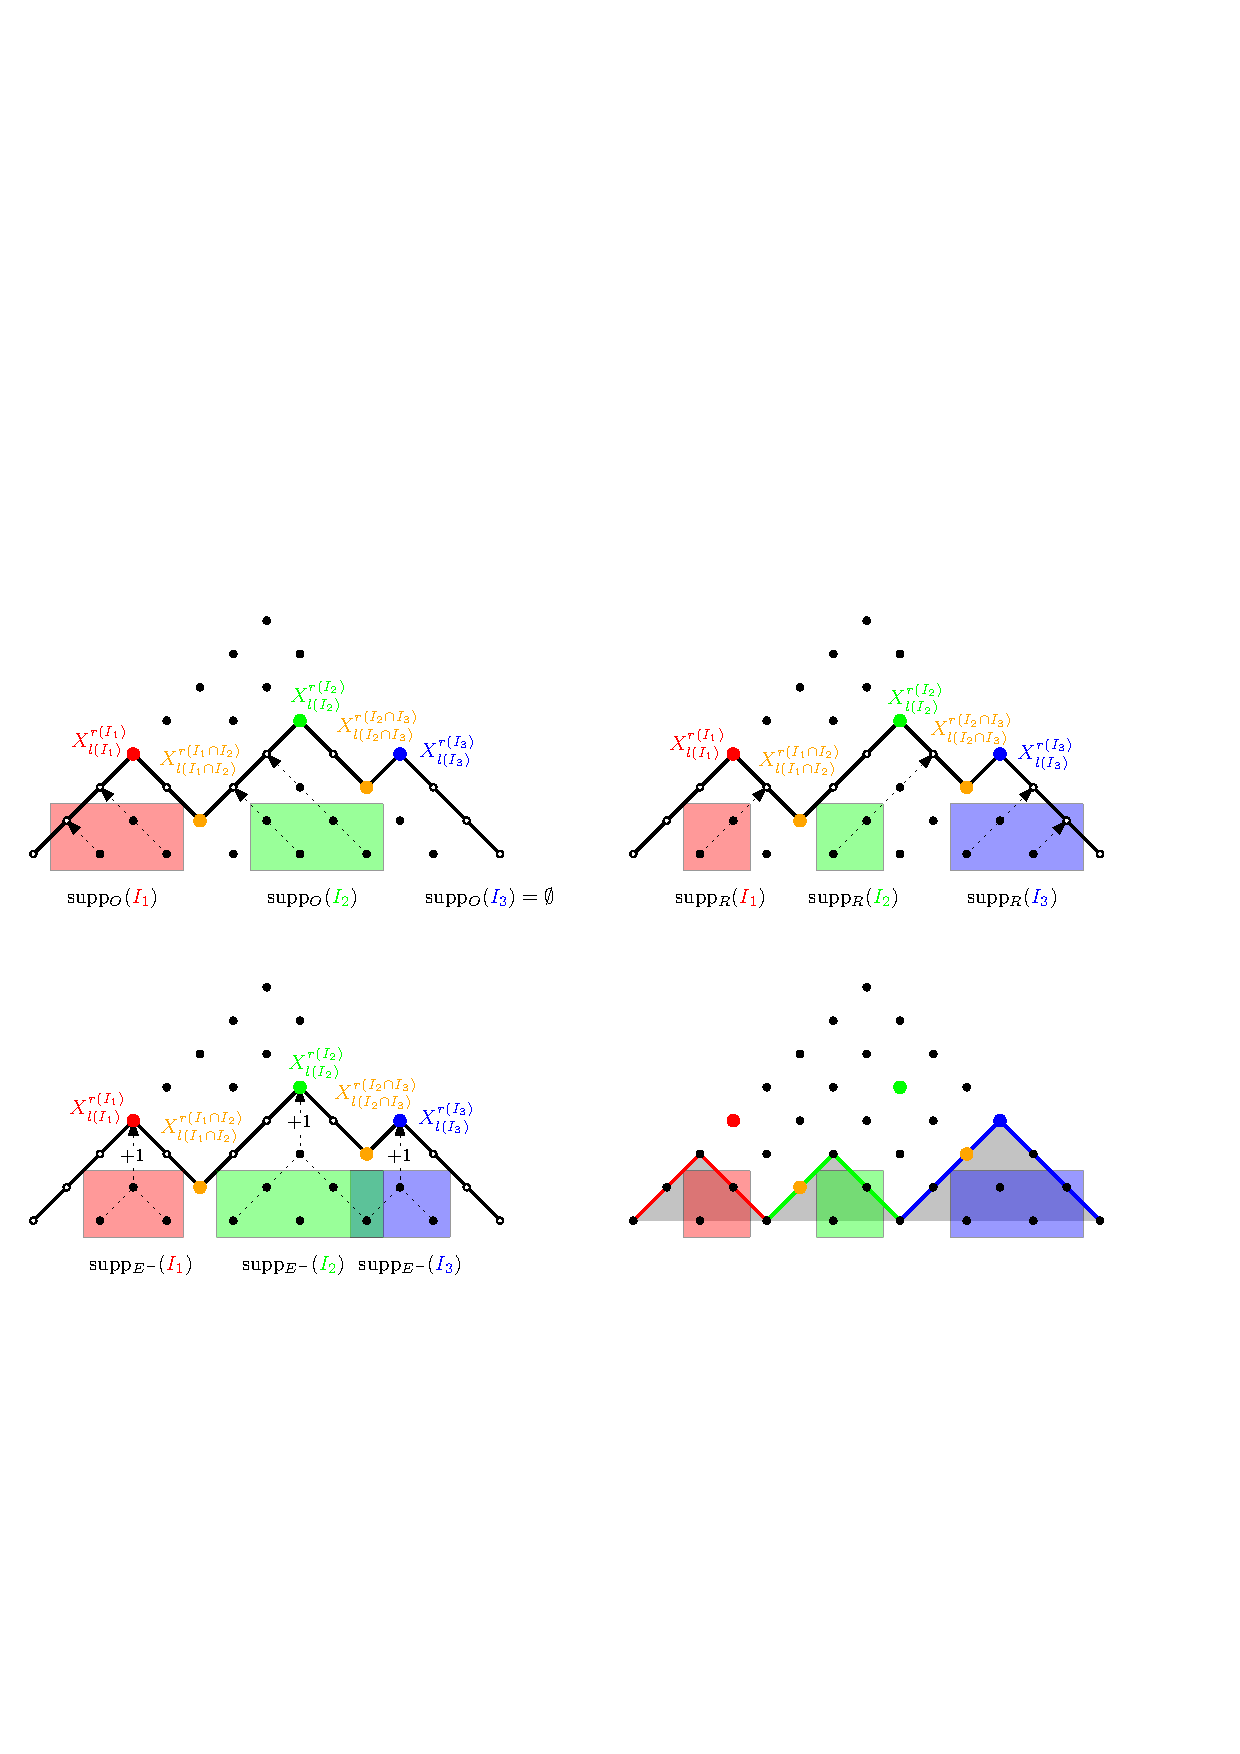
\includegraphics[width=15cm]{figures/ZZProjections}
\caption[Zigzag persistence modules in the half-pyramid]{\label{fig:suppZZ} The black path in the south face of the
  Mayer-Vietoris half-pyramid represents the monotone zigzag persistence module
  $\overline{\rm CZZ}(f,\mathcal I)$ for a gomic $\I$ with three intervals. The
  white disks on this path are the nodes that do not intersect the set
  of nodes of the cover zigzag persistence module $\CZZ(f,\I)$, which are colored
  according to the interval of $\I$ they represent (and are colored
  orange if they represent an intersection). The boxes outline the
  support of the intervals of $\DgZZ_0(f)$ that disappear in the
  MultiNerve Mapper depending on their types (upper-left for
  type I intervals, upper-right for type II intervals and
  down-left for type IV intervals). We also show (down-right) the
  analogue, drawn in grey color, of $Q^{\I}_R$ on the south face of the
  Mayer-Vietoris half-pyramid.}
\end{figure}

There are two possible ways for an interval of $\DgZZ_0(f)$ to disappear in $\DgCZZ_0(f,\I)$: 
either its homological dimension is shifted by 1, or its intersection with the set of nodes of $\CZZ(f,\I)$ is empty
after being projected onto $\overline\DgCZZ_0(f,\I)$---see Figure~\ref{fig:suppZZ}.
%The following items are consequences of 
According to the pyramid rules, we have that:
\begin{itemize}
\item Projections of type III intervals of $\DgZZ_0(f)$ onto $\overline\DgCZZ_0(f,\I)$ always intersect with the nodes of $\CZZ(f,\I)$
and their homological dimensions cannot be shifted.
Hence, none of them disappears. This proves (iv).
\item Projections of type IV intervals of $\DgZZ_0(f)$ onto $\overline\DgCZZ_0(f,\I)$ always intersect with the nodes of $\CZZ(f,\I)$.
However, their homological dimensions can be shifted by 1.
This happens when the endpoints collide in the south face of the Mayer-Vietoris half-pyramid. Hence, only those intervals whose support 
is included in ${\rm supp}_{E^-}(I)$ for some $I\in\I$
go through such a shift before getting to $\overline\DgCZZ_0(f,\I)$. This proves (iii).
\item Homological dimensions of type I intervals in $\DgZZ_0(f)$ cannot be shifted, but their projections onto $\overline\DgCZZ_0(f,\I)$ may 
not always intersect with the nodes of $\CZZ(f,\I)$.
This happens for those intervals whose support is included in ${\rm supp}_{O}(I)$ for some $I\in\I$, thus proving (i). 
\item Homological dimensions of type II intervals in $\DgZZ_0(f)$ cannot be shifted, but their projections onto $\overline\DgCZZ_0(f,\I)$ may
not always intersect with the nodes of $\CZZ(f,\I)$. 
This happens for those intervals whose support is included in ${\rm supp}_{R}(I)$ for some $I\in\I$, thus proving (ii). 
\end{itemize}
\end{proof}


\subsection{A signature for MultiNerve Mapper} 
\label{sec:MultiNerveSign}

Theorem~\ref{th:ExDgMultiNerve} means that the dictionary
introduced in Section~\ref{sec:dictionary} can be used to describe
the structure of the MultiNerve Mapper from the extended persistence
diagram of the induced function~$\tilde f$. 
Indeed, the topological features of $\MMapper_f(X,\I)$
are in bijection with the points of
$\Dg(\tilde f)$ minus the ones that fall into the various
staircases ($Q_O^{\I}$, $Q_{E^-}^{\I}$, $Q_R^{\I}$) corresponding to their type. 
Moreover, by Theorem~\ref{thm:pdreeb}, $\Dg(\tilde f)$ itself is
obtained from $\Dg_0(f)$ and $\Dg_1(f)$ by removing the points of
$\Ext_1^+(f)$ and $\Ord_1(f)$.
%To avoid the arbitrary choice of $f_{\I}$,
Hence, we use the off-staircase part of
$\Dg(\tilde f)$ as a signature for the structure of the MultiNerve
Mapper\footnote{Recall that $\Ext_0^-(f)=\Rel_0(f)=\emptyset$.}:
%
\begin{align}\label{eq:sign1}
\begin{split}
\Dg(\MMapper_f(X,\I))&=
(\Ord(\tilde{f})\setminus Q_O^{\I})\cup
(\Ext(\tilde{f})\setminus Q_{E^-}^{\I})\cup
(\Rel(\tilde{f})\setminus Q_R^{\I})\\
&=
(\Ord_0(f)\setminus Q_O^{\I})\cup
((\Ext_0^+(f)\cup \Ext_1^-(f))\setminus Q_{E^-}^{\I})\cup
(\Rel_1(f)\setminus Q_R^{\I}).
\end{split}
\end{align}
%
We call this signature the {\em extended persistence diagram} of the MultiNerve Mapper.  
Note that this signature is not computed by applying persistence
to some function defined on the multinerve, but it is rather
a pruned version of the extended persistence diagram of ${\tilde f}$. 
As for Reeb graphs,
it serves as a bag-of-features type signature of the structure of
$\MMapper_f(X, \I)$. 
%
Moreover, the fact that $\Dg(\MMapper_f(X, \I)) \subseteq \Dg(\tilde
f)$ formalizes the intuition that the MultiNerve Mapper should be
viewed as a {\em pixelized version} of the Reeb graph, in which some
of the features disappear due to the staircases (prescribed by the cover). 
%
For instance, in Figure~\ref{fig:ExDict} we show a double torus
equipped with the height function, together with its associated Reeb
graph, MultiNerve Mapper, and Mapper. We also show the corresponding
extended persistence diagrams.  In each case, the points in the diagram
represent the features of the object: the extended points represent
the holes (dimension 1 and above) and the trunks (dimension 0) while
the ordinary and relative points represent the branches.

\begin{figure}[h]
\centering
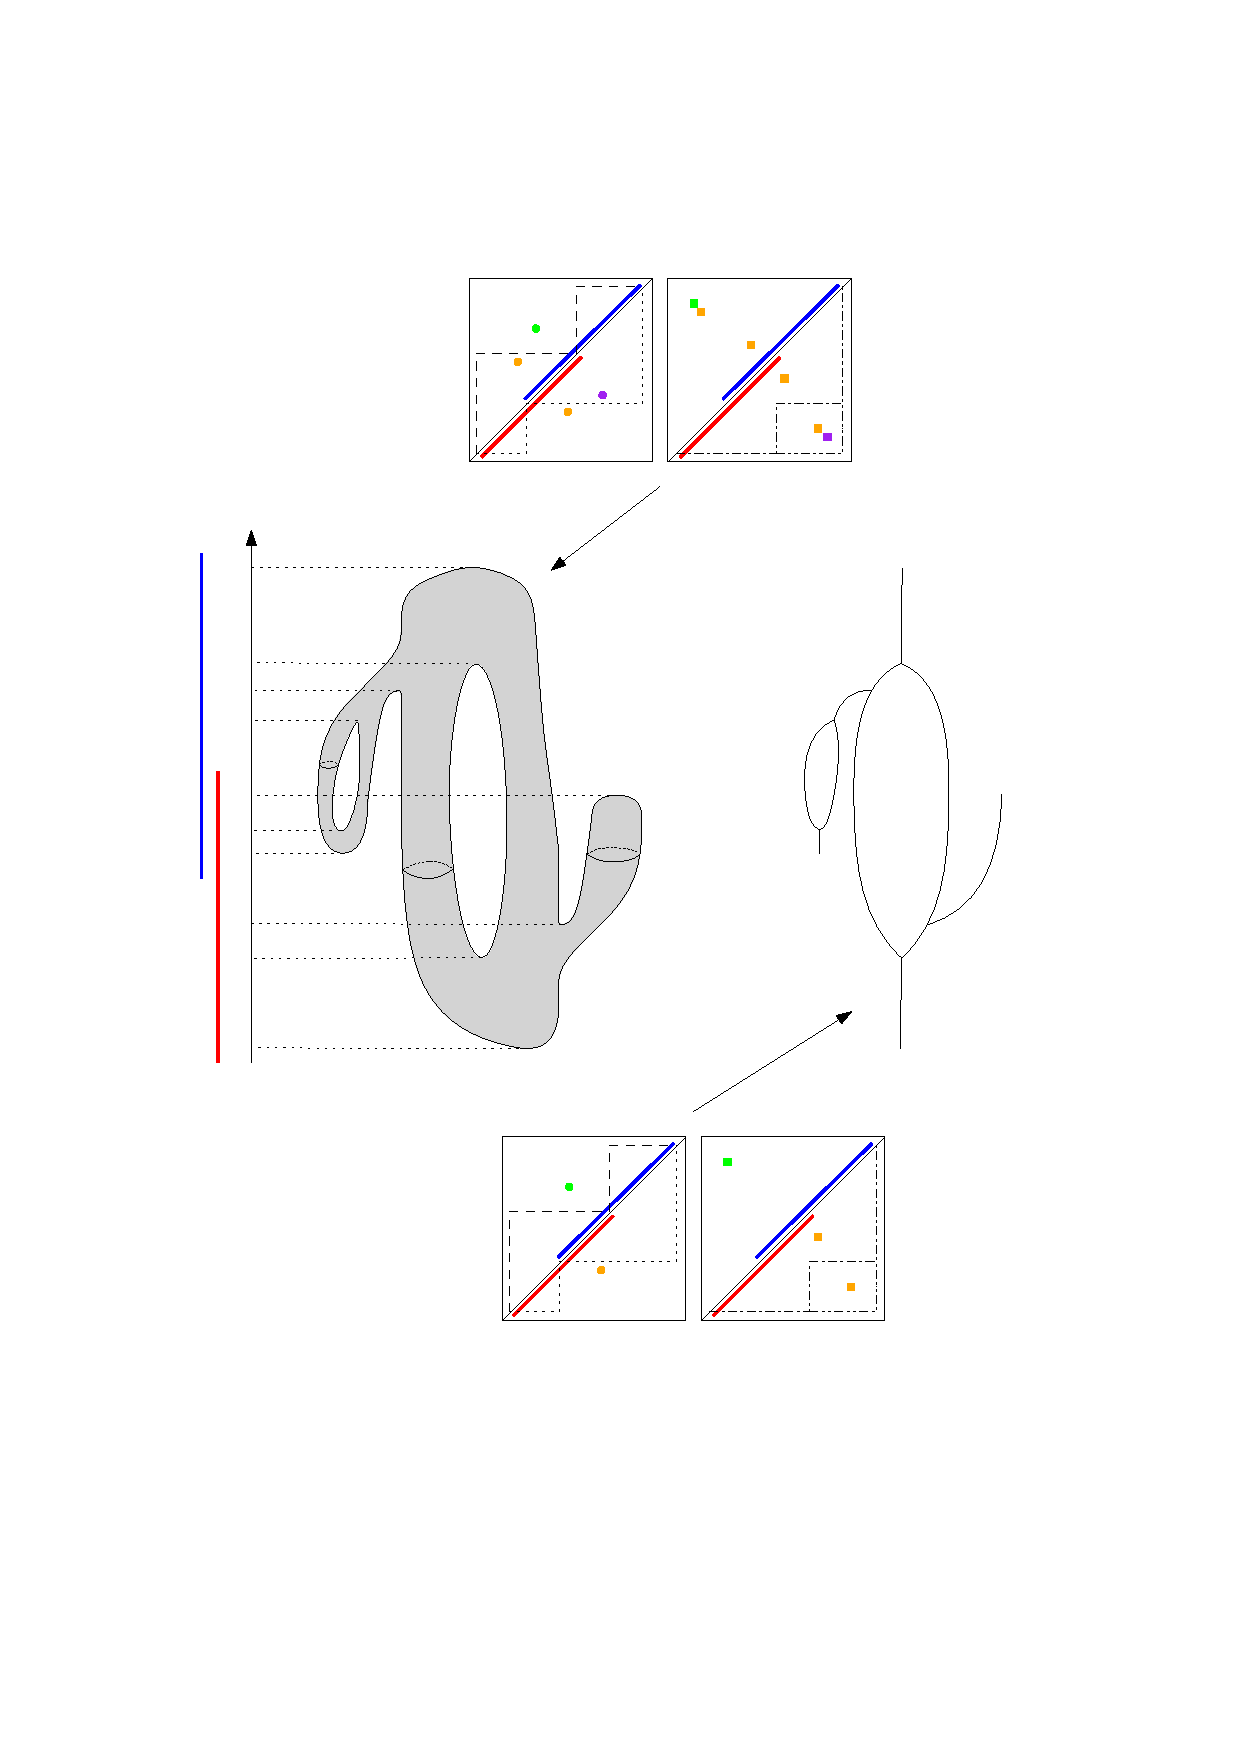
\includegraphics[height=10cm]{figures/ExDict1}\ \ \ \ \ \ \ \ 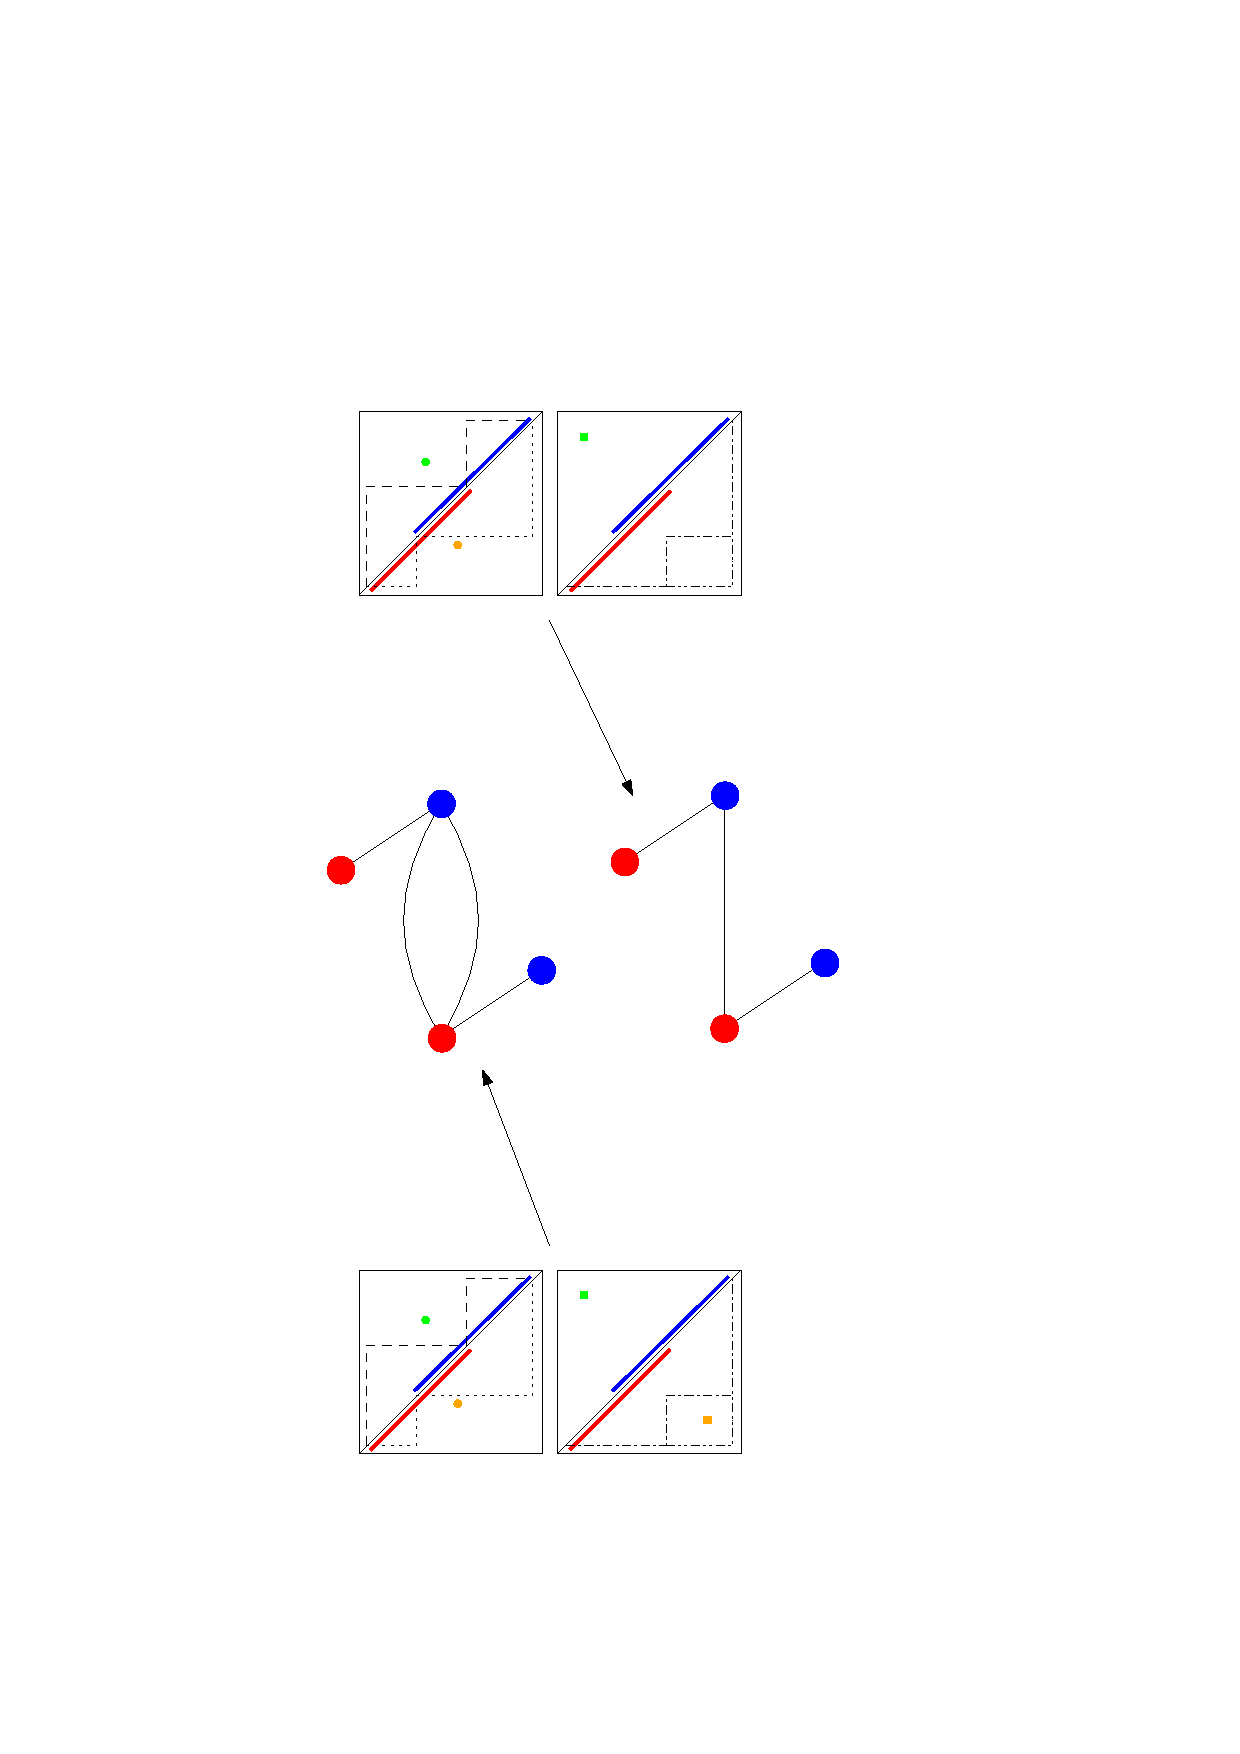
\includegraphics[height=10cm]{figures/ExDict2}
\caption[Mapper as a pixelization of the Reeb graph]{From left to right: a 2-manifold equipped with the height
  function; the corresponding Reeb graph, MultiNerve Mapper, and
  Mapper. For each object, we display the extended persistence diagrams of
  dimension 0 (green points), 1 (orange points) and 2 (purple
  points). Extended points are squares while ordinary and relative
  points are disks (above and below the diagonal respectively).  The
  staircases are represented with dashed ($Q_O^{\I}$), dotted ($Q_{E^-}^{\I}$),
  dash-dotted ($Q_R^{\I}$), and dash-dot-dotted ($Q_{E}^{\I}$) lines.  
  One can see how to go from the extended
  persistence diagram of the height function to the one of the induced map
  (remove the points in dimension 2 and the points in dimension 1
  above the diagonal), then to the one of the MultiNerve Mapper
  (remove the points inside the staircases corresponding to their
  type), and finally, to the one of the Mapper (remove the extended
  points in $Q_{E}^{\I}$).}
\label{fig:ExDict}
\end{figure}



\paragraph*{Convergence of the signature.} The following convergence
result (which is in fact non-asymptotic) is a direct consequence of
our previous results:
%
\begin{cor}\label{cor:Reeb_approx}
Suppose the granularity of the gomic~$\I$ is at most $\e$. Then, 
%
\[
 \Dg(\tilde f)\setminus \{(x,y) \,:\, |y-x|\leq \e\} \subseteq \Dg(\MMapper_f(X, \I)) \subseteq \Dg(\tilde f).
\]
%
Thus, the features (branches, holes) of the Reeb graph that are
missing in the MultiNerve Mapper have spans at most~$\e$.  In
particular, we have $\distb(\Dg(\MMapper_f(X, \I)),
\Dg(\tilde f))\leq \e/2$.  Moreover, the two signatures become equal
when $\e$ becomes smaller than the smallest vertical distance of the
points of $\Dg(\tilde f)$ to the diagonal. Finally, $\MMapper_f(X,
\I)$ and $\Reeb_f(X)$ themselves become isomorphic as combinatorial graphs up to
one-step vertex splits and edge subdivisions (which are
topologically trivial modifications)
when $\e$ becomes smaller than the smallest absolute difference
between distinct critical values of~$f$.
\end{cor}
%
We show a similar convergence
result in the functional distortion distance in Section~\ref{sec:stabdfd}.
Note that building the signature $\Dg(\MMapper_f(X, \I))$
requires computing the critical values of~$f$ exactly, which may not
always be possible. However, as for Reeb graphs, the signature can be
approximated efficiently and with theoretical guarantees under mild
sampling conditions using existing work on scalar fields analysis, as
we will see in Chapter~\ref{chap:MapperStatistic}. %Section~\ref{sec:discrete}. 


\subsection{Induced signature for Mapper}
\label{sec:MapperSign} 

Recall from Lemma~\ref{lem:pi1_surj} that the projection
$\pi_1:\MMapper_f(X,\I)\to \Mapper_f(X,\I)$ induces a surjective
homomorphism in homology. Thus, the Mapper has a simpler structure
than the MultiNerve Mapper. To be more specific, $\pi_1$ identifies all the 
edges connecting the same pair of vertices. This eliminates the corresponding 
holes in $\MMapper_f(X,\I)$. Since the two vertices
lie in successive intervals of the cover, the corresponding diagram points lie 
in the following extended staircase 
(see the staircase $Q^{\I}_E$ displayed on the right in Figure~\ref{fig:staircase}):
%
\[
\StairExtM=\bigcup_{I\cup J \text{ such that } I\cap J\neq \emptyset}Q_{I\cup J}^-.
\]
%
The other staircases remain unchanged. Hence the following signature:
%
\begin{align}\label{eq:sign_Mapper}
\begin{split}
\Dg(\Mapper_f(X,\I))&=
(\Ord(\tilde{f})\setminus Q_O^{\I})\cup
(\Ext(\tilde{f})\setminus Q_{E}^{\I})\cup
(\Rel(\tilde{f})\setminus Q_R^{\I})\\
&=
(\Ord_0(f)\setminus Q_O^{\I})\cup
((\Ext_0^+(f)\cup \Ext_1^-(f))\setminus Q_{E}^{\I})\cup
(\Rel_1(f)\setminus Q_R^{\I}).
\end{split}
\end{align}
%
The interpretation of this signature in terms of the structure of the
Mapper follows the same rules as for the MultiNerve Mapper and Reeb
graph---see again Figure~\ref{fig:ExDict}.
Moreover, the convergence result stated in
Corollary~\ref{cor:Reeb_approx} holds for the Mapper as well.



















%%%%%%%%%
\section{Stability in the bottleneck distance}
%\label{sec:Stability}
\label{sec:Stab_func}

Intuitively, for a point in the signature $\Dg(\MMapper_f(X,\I))$,
the $\ell^\infty$-distance to its corresponding
staircase\footnote{$Q_O^{\I}$, $Q_{E^-}^{\I}$ or $Q_R^{\I}$, depending on the type of the point.}  
measures the amount by which the
function~$f$ or the cover~$\I$ must be perturbed in order to eliminate
the corresponding feature (branch, hole) in the MultiNerve
Mapper. Conversely, for a point in the Reeb graph's signature
$\Dg(\tilde f)$ that is not in the MultiNerve Mapper's signature
(i.e. that lies inside its corresponding staircase), the
$\ell^\infty$-distance to the boundary of the staircase measures the
amount by which~$f$ or~$\I$ must be perturbed in order to create a
corresponding feature in the MultiNerve Mapper. Our goal here is to
formalize this intuition. For this we adapt the bottleneck distance so
that it takes the staircases into account. Our results are stated for
the MultiNerve Mapper, they hold the same for the Mapper with the
staircase $Q_{E^-}^{\I}$ replaced by its extension $Q_{E}^{\I}$.
%We detail three types of stability: one with respect to perturbations of the functions in Section~\ref{sec:Stab_func},
%one with respect to perturbations of the domains in Section~\ref{sec:Stab_domain},
%and one with respect to perturbations of the covers in Section~\ref{sec:Stab_cover}.

\paragraph*{An extension of the bottleneck distance.} Let $\Theta$ be a subset of
$\R^2$. Given a partial matching $\Gamma$ between two extended persistence
diagrams $\Dg, \Dg'$, the \emph{$\Theta$-cost} of $\Gamma$ is:
%
\[
\mathrm{cost}_\Theta(\Gamma)=\max\left\{\max_{p\in \Dg}\ \delta_{\Dg}(p),\ \max_{p'\in {\Dg'}}\ \delta_{\Dg'}(p')\right\},
\]
%
where:
%
\[
\delta_{\Dg}(p)=\|p-p'\|_\infty \text{ if } \exists p'\in \Dg'\text{ such that }(p,p')\in\Gamma \text{ and } d_\infty(p,\Theta) \text{ otherwise},
\]
\[
\delta_{\Dg'}(p')=\|p-p'\|_\infty \text{ if } \exists p\in \Dg\text{ such that }(p,p')\in\Gamma \text{ and } d_\infty(p',\Theta) \text{ otherwise}.
\]
%
The bottleneck distance becomes:
%
\[
\diststair(\Dg,\Dg')=\inf_{\Gamma}\ \mathrm{cost}_\Theta(\Gamma),
\]
%
where $\Gamma$ ranges over all partial matchings between $\Dg$ and
$\Dg'$. This is again a pseudometric and not a metric. 
%To avoid heavy notations, we write $d_\Theta$ instead of $d^\infty_{\text{b},\Theta}$. 
Note that the usual bottleneck distance
is obtained by taking $\Theta$ to be the diagonal $\Diag$.  
%
Given a gomic $\I$, we choose different sets $\Theta$ depending on the
types of the points in the two diagrams. More precisely, we define the
distance between signatures as follows:

\begin{defin}
Given a gomic $\I$, we define the distance $d_{\mathcal I}$ between extended persistence diagrams $\Dg,\Dg'$ as:
\begin{equation}\label{eq:def-bottleneck-MMapper} 
\distcov(\Dg,\Dg')=\max\left\{
d_{\rm{b},Q_O^{\I}}(\Ord, \Ord'),\; 
d_{\rm{b},Q_{E^-}^{\I}}(\Ext, \Ext'),\; 
d_{\rm{b},Q_R^{\I}}(\Rel, \Rel') \right\}. 
\end{equation}
\end{defin}










%\subsection{Stability with respect to perturbations of the function}


The distance $d_{\I}$ {\em stabilizes} the (MultiNerve) Mappers, as stated in the following theorem:

\begin{thm}\label{thm:MStab}
Given a topological space $X$, Morse-type functions $f,g:X\to\R$ and a gomic $\I$ of granularity at most $\epsilon > 0$, 
the following stability inequality holds:
%
\begin{align}
&d_{\I}(\Dg(\Mapper_f(X,\I)),\Dg(\Mapper_g(X,\I))) \leq d_{\I}(\Dg(\MMapper_f(X,\I)),\Dg(\MMapper_g(X,\I))) \leq \|f-g\|_\infty. \label{ineq:stabilitydi}
\end{align}

Moreover, $d_{\I}$ and $\distb$ are related as follows:
%
\begin{align}
&\distb(\Dg(\MMapper_f(X,\I)),\Dg(\MMapper_g(X,\I))) \leq \frac \e2 + d_{\I}(\Dg(\MMapper_f(X,\I)),\Dg(\MMapper_g(X,\I))).\label{ineq:didbMM}\\
&\distb(\Dg(\Mapper_f(X,\I)),\Dg(\Mapper_g(X,\I))) \leq \e + d_{\I}(\Dg(\Mapper_f(X,\I)),\Dg(\Mapper_g(X,\I))).\label{ineq:didbM}
\end{align}
%
\end{thm}
%
Note that Theorem~\ref{thm:MStab} can be readily extended to Morse-type functions with different domains using results in~\cite{Carriere15b}.
In that case, the upper bound depends on the Gromov-Hausdorff distance between the domains. 
%
\begin{figure}[t]\begin{center}
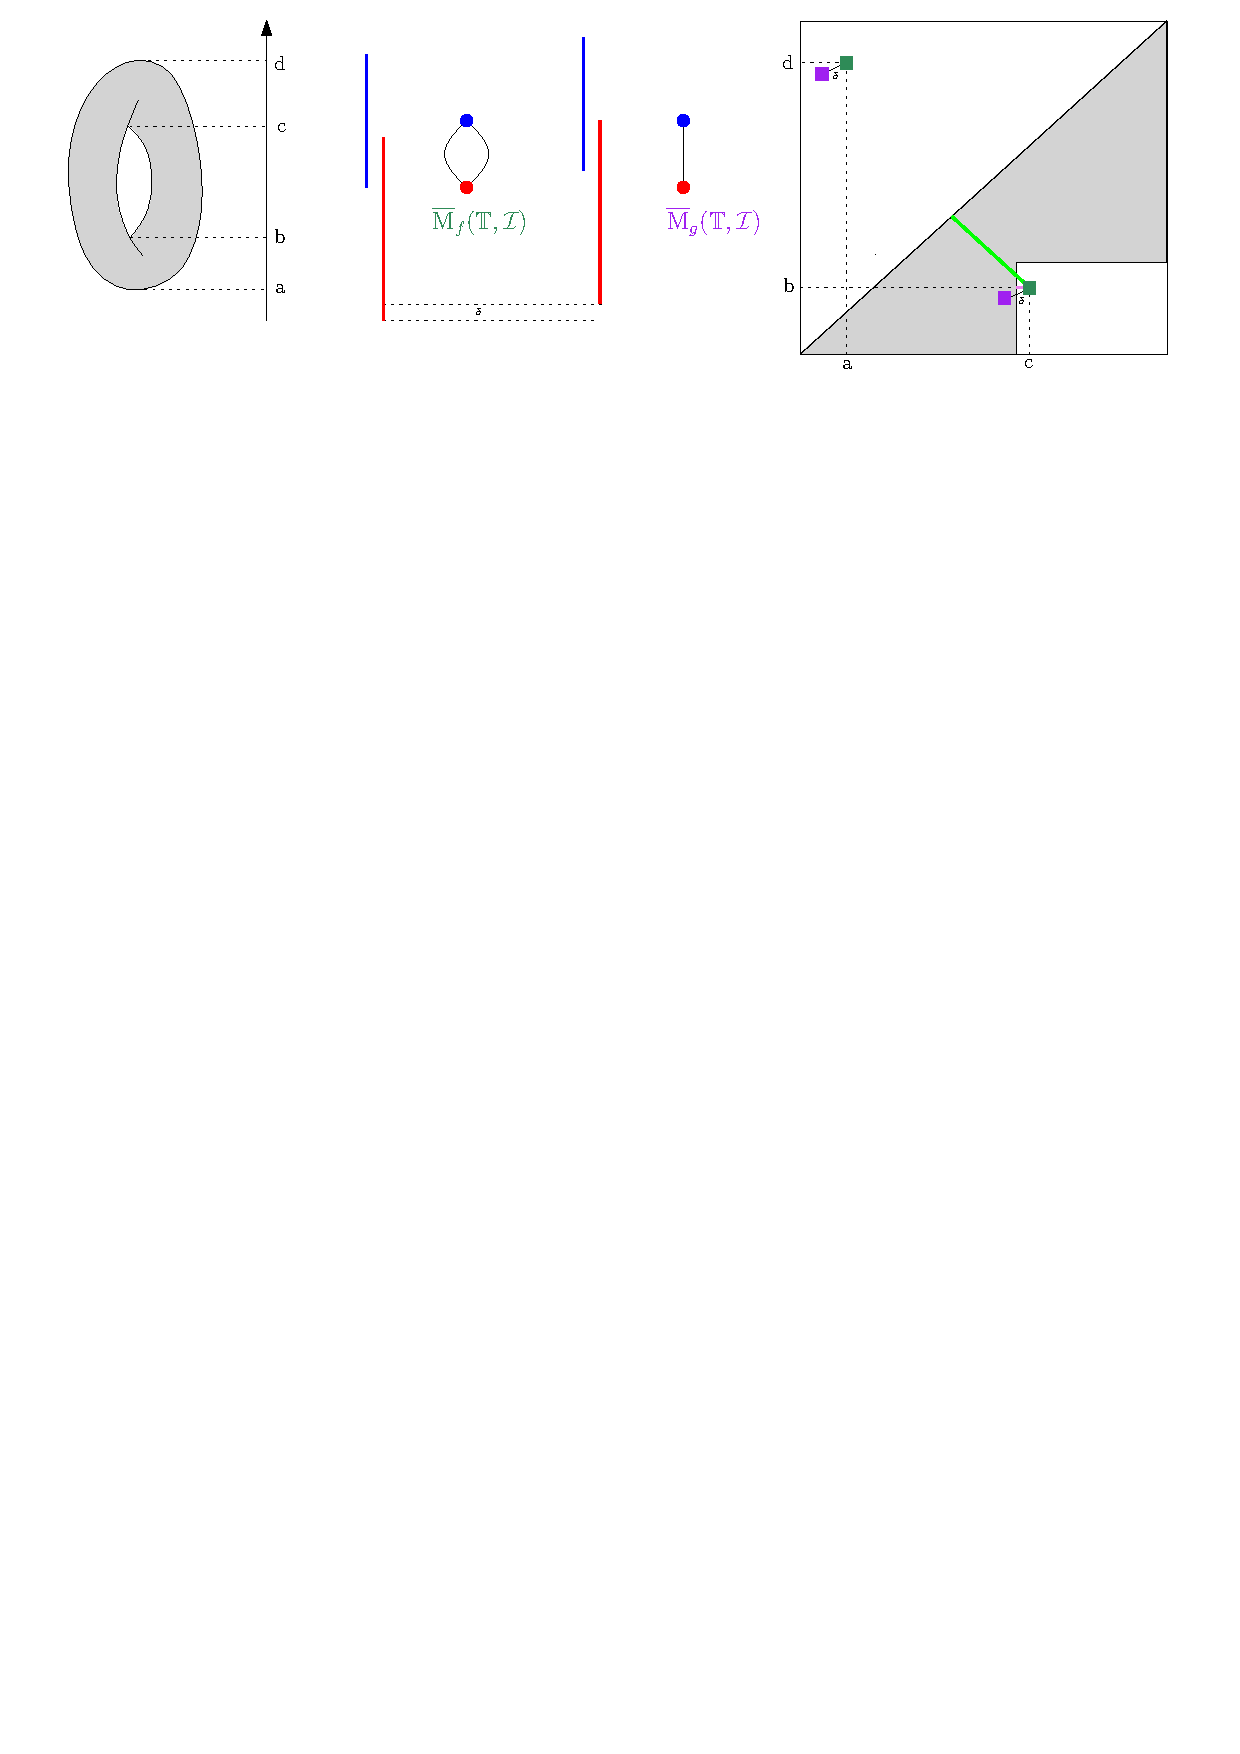
\includegraphics[height=4cm]{figures/InstabBottleneck}
\caption[Stability of the Mapper]{\label{fig:counterexample} We compute the MultiNerve Mapper of the height function $f$ on the torus $\T$,
given a gomic $\I$ with two intervals.
We also compute the MultiNerve Mapper of a perturbed function $g$ such that $\|f-g\|_\infty\leq\delta$.
We plot the extended persistence diagrams of $\tilde f$ (dark green) and $\tilde g$ (purple). Note that the signature of $\MMapper_g(\T,\I)$
is obtained by removing the purple point beneath the diagonal since it belongs to a staircase, while the signature of $\MMapper_f(\T,\I)$
is equal to $\Dg({\tilde f})$. If we used the bottleneck distance to compare the two signatures, their distance would be equal to
the distance to the diagonal of the dark green point beneath $\Diag$ (green segment), which can be arbitrarily large, while, using 
$d_{\I}$, their distance becomes the distance of the
same point to the staircase (tiny pink segment), which is bounded by $\delta$.}
\end{center}\end{figure}
%

The proof of Theorem~\ref{thm:MStab} relies on the following monotonicity
property, which is immediate:
%
\begin{lem}\label{lem:ineqsub}
Let $\Theta\subseteq\R^2$ be in the closure of $\Theta'\subseteq\R^2$. 
Then, $$d_{\Theta'}(\Dg,\Dg')\leq d_\Theta(\Dg,\Dg')\leq d_{\Theta'}(\Dg,\Dg')+\disth(\Theta,\Theta'),$$
where $\disth$ denotes the Hausdorff distance in the $\ell_\infty$-norm.
\end{lem}

\begin{proof}[Proof of Theorem~\ref{thm:MStab}]
Equation~(\ref{ineq:didbMM}) and~(\ref{ineq:didbM}) are direct applications of Lemma~\ref{lem:ineqsub}.
Equation~(\ref{ineq:stabilitydi}) is proven by the following sequence of (in)equalities:
%
\begin{align*}
d_{\I}(\Dg(\MMapper_f(X,\I)),\Dg(\MMapper_g(X,\I))) &=d_{\I}(\Dg(\tilde f), \Dg(\tilde g))\\
&\leq d_{\rm{b},\Diag}(\Dg(\tilde f), \Dg(\tilde g))=\distb(\Dg(\tilde f), \Dg(\tilde g))\\
&\leq \distb(\Dg(f),\Dg(g))\\
&\leq \|f-g\|_\infty.
\end{align*}
%
The first equality comes from the observation that the points
of $\Dg(\tilde f)\sqcup\Dg(\tilde g)$ that lie inside
their corresponding staircase can be left unmatched and have a zero
cost in the matching, so removing them as in~(\ref{eq:sign1}) does not change the bottleneck cost. 
The first inequality follows from Lemma~\ref{lem:ineqsub} since the diagonal $\Diag$ is included in the closure of each of the staircases. 
The second inequality follows from Theorem~\ref{thm:pdreeb} and the fact that the matchings only match points of 
the same type (ordinary, extended, relative) and of the same homological dimension. The last inequality comes from  Theorem~\ref{th:ExStab}.
\end{proof}

\paragraph*{Interpretation of the stability.} Note that the bottleneck distance $\distb$ is unstable in this context---see Figure~\ref{fig:counterexample}. 
The theorem allows us to make some interesting claims. 
For instance, denoting by $Q_p^{\I}$ the staircase corresponding to the type of a diagram point~$p$,  the quantity 
%
\[
d_{\I}(\Dg, \emptyset) = \max_{p\in \Dg} d_\infty(p, Q_p^{\I}) 
\]
%
measures the amount by which the diagram~$\Dg$ must be perturbed in the
metric~$d_{\I}$ in order to bring all its points to the staircase. Hence, by Theorem~\ref{thm:MStab}, given a pair~$(X,f)$, the quantity 
%
\[
d_{\I}(\Dg(\MMapper_f(X,\I)), \emptyset) = \max_{p\in \Dg(\MMapper_f(X,\I))} d_\infty(p, Q_p^{\I}) 
\]
%
is a lower bound on the amount by which $f$ must be perturbed in
the supremum norm in order to remove all the features (branches and
holes) from the MultiNerve Mapper. Conversely, 
%
\[
\min_{p\in \Dg(\MMapper_f(X,\I))} d_\infty(p, Q_p^{\I}) 
\]
%
is a lower bound on the maximum amount of perturbation allowed for~$f$
if one wants to preserve all the features in the MultiNerve
Mapper no matter what. Note that this does not prevent other features from
appearing. The quantity that controls those is related to the
points of~$\Dg(\tilde f)$ (including 
diagonal points) that lie in the staircases. More precisely, the quantity
%
\[%begin{equation}\label{eq:perturb_min}
\min_{p\in \Dg(\tilde f) \cup \Delta} d_\infty(p, \partial Q_p^{\I}\setminus\Delta)
\]%end{equation}

is a lower bound on the maximum amount by which $f$ can be perturbed
if one wants to preserve the structure (set of features) of the
MultiNerve Mapper no matter what. Note that this lower bound is
in fact zero since $\partial Q_O^{\I}\setminus\Diag$ and $\partial
Q_R^{\I}\setminus\Diag$ come arbitrarily close to the diagonal~$\Delta$
(recall Figure~\ref{fig:staircase}). This means that, as small as the
perturbation of~$f$ may be, it can always make new branches appear in
the MultiNerve Mapper. However, it will not impact the set of holes if
its amplitude is less than
%
\[
\min_{p\in \Ext(\tilde f) \cup \Delta} d_\infty(p, \partial Q_{E^-}^{\I}\setminus\Delta).
\]
%
From this discussion we derive the following rule of thumb: having
small overlaps between the intervals of the gomic helps capture more
features (branches and holes) of the Reeb graph in the (MultiNerve)
Mapper; conversely, having large overlaps helps prevent new holes from
appearing in the (MultiNerve) Mapper under small perturbations of the
function. This is an important trade-off to consider in applications.



%\subsection{Stability with respect to perturbations of the domain}
%\label{sec:Stab_domain}

%More generally, we can derive a stability result for perturbations of
%the pair $(X,f)$, provided we make some extra assumptions on the
%regularity of the domain and function. 

%\paragraph*{Convention.} In this Section, we assume $X$
%to be a compact Riemannian manifold (or, more generally, a compact
%length space with curvature bounded above) and $f$ to be
%Lipschitz-continuous. 

%\paragraph*{The Gromov-Hausdorff distance for metric spaces.} To measure the amount of perturbation of the
%domain we use the concept of {\em correspondence} from metric
%geometry: given another pair $(Y,g)$, a correspondence is a subset~$C$
%of the product space $X\times Y$ such that the canonical projections
%$C\to X$ and $C\to Y$ are surjective.  We consider the {\em functional
%  distortion} associated with~$C$, which is the quantity:
% 
%\[
%\e_{\mathfrak{f}}(C) = \sup_{(x,y)\in C} |f(x)-g(y)|.
%\]
%
%Similarly, writing respectively $d_X$ and $d_Y$ for the intrinsic
%metrics of $X$ and $Y$, we consider the {\em metric distortion} of~$C$:
%
%\[
%\e_{\mathfrak{m}}(C) = \sup_{(x,y)\in C, (x',y')\in C} |d_X(x,x')-d_Y(y,y')|.
%\]
%
%The {\em Gromov-Hausdorff distance} between $X$ and $Y$ is then:
%
%\begin{equation}
%d_{\text{GH}}(X,Y) = \frac{1}{2}\inf_C \e_{\mathfrak{m}}(C),
%\end{equation}
%
%where $C$ ranges over all correspondences between $X$ and $Y$. Now we
%can derive a stability guarantee for the descriptors of MultiNerve
%Mappers in this context, using a variant of Theorem~\ref{th:ExStab}
%proven in~\cite{Carriere15b}:
%
%\begin{thm}\label{thm:DStab}
%Fix a gomic~$\I$. Let $X$ and $Y$ be two compact Riemannian manifolds
%or length spaces with curvature bounded above.  Denote by $\rho(X)$
%and $\rho(Y)$ their respective convexity radii.  Let
%$f:X\rightarrow\R$ and $g:Y\to\R$ be Lipschitz-continuous Morse-type
%functions, with Lipschitz constants $c_f$ and $c_g$ respectively.
%Assume $d_\emph{GH}(X,Y)\leq\frac{1}{20}\,\min(\rho(X),\rho(Y))$.
%Then, for any correspondence $C\in\mathcal{C}(X,Y)$ such that
%$\epsilon_{\mathfrak{m}}(C)<\frac{1}{10}\,\min(\rho(X),\rho(Y))$,
%
%\[
%d_{\I}(\Dg(\MMapper_f(X,\I)),\Dg(\MMapper_g(Y,\I)))\leq (9(c_f+c_g)+\min\{c_f,c_g\})\epsilon_{\mathfrak{m}}(C)+\epsilon_{\mathfrak{f}}(C).
%\]
%
%\end{thm}
%
%\begin{proof}
%The proof is the same sequence of (in)equalities as for
%Theorem~\ref{thm:MStab}, except the last inequality is replaced by
%$\distb(\Dg(f),\Dg(g))\leq
%(9(c_f+c_g)+\min\{c_f,c_g\})\epsilon_{\mathfrak{m}}(C)+\epsilon_{\mathfrak{f}}(C)$, which comes\footnote{Note
%  that Theorem~3.4 in~\cite{Carriere15b} is stated only for the ordinary part of
%  the persistence diagrams, however its analysis extends to the
%  full extended filtrations at no extra cost.} from Theorem~3.4
%in~\cite{Carriere15b}.
%\end{proof}

%This result brings about the same discussion as in
%Section~\ref{sec:Stab_func}, with $f$ replaced by the pair~$(X,f)$.


\section{Stability with respect to perturbations of the cover}
\label{sec:Stab_cover}

Let us now fix the pair $(X,f)$ and consider varying gomics.  For each
choice of gomic, 
Eqs.~(\ref{eq:sign1})-(\ref{eq:sign_Mapper}) tell which points
of the diagram~$\Dg(f)$ end up in the diagram of the (MultiNerve)
Mapper and thus participate in its structure. We aim for a
quantification of the extent to which this structure may change as the
gomic is perturbed.  For this we adopt the dual point of view: for any
two choices of gomics, we want to use the points of the
diagram~$\Dg(f)$ to assess the degree by which the gomics differ.
This is a reversed situation compared to Section~\ref{sec:Stab_func},
where the gomic was fixed and was used to assess the degree by which
the persistence diagrams of two functions differed.

\paragraph*{A distance between gomics.} The diagram points that discriminate between the two gomics are the
ones located in the symmetric difference of the staircases, since they
witness that the symmetric difference is
non-empty. Moreover, their $\ell^\infty$-distances to the staircase of
the other gomic provide a lower bound on the Hausdorff distance
between the two staircases and thus quantify the extent to which the
two covers differ. We formalize this intuition as follows: given a
persistence diagram~$\Dg$ and two gomics $\I, \J$, we consider the
quantity:
%
\begin{equation}\label{eq:def-dist-covers}
d_{\Dg}(\I, \J) = \max_{*\in \{O, {E^-}, R\}}
\left\{ \sup_{p\in \Dg^*\cap (Q_*^{\I} \symdiff Q_*^{\J})} \max\left\{ d_\infty(p, Q_*^{\I}),\, d_\infty(p, Q_*^{\J})\right\}
\right\},
\end{equation}
% 
where $\symdiff$ denotes the symmetric difference, where $\Dg^*$ stands
for the subdiagram of $\Dg$ of the right type ($\Ord$, $\Ext$ or
$\Rel$), and where we adopt the convention that $\sup_{p\in
  \emptyset} ... $ is zero instead of infinite.  Note that there is
always one of the two terms in (\ref{eq:def-dist-covers}) that is zero
since the supremum is taken over all points that lie in the symmetric
difference of the staircases.  Deriving an upper bound on $d_{\Dg}(\I,\J)$ 
in terms of the Hausdorff distances between the staircases is
straightforward, since the supremum in~(\ref{eq:def-dist-covers}) is
taken over points that lie in the symmetric difference between the
staircases:

\[%begin{equation}\label{eq:dist-covers-bound}
d_{\Dg}(\I, \J) \leq \max_{*\in \{O, {E^-}, R\}} \disth(Q_*^{\I},\, Q_*^{\J}),
\]%end{equation}
%
where $\disth$ stands for the Hausdorff distance in the $\ell^\infty$-norm.
%\end{lem}
%
The connection to the MultiNerve Mapper appears when we take $\Dg$ to be the
persistence diagram of the induced map~$\tilde f$ defined on the Reeb
graph $\Reeb_f(X)$. Indeed, we have
%
\[
\Ord(\tilde f)\cap (Q_O^{\I} \symdiff Q_O^{\J}) = (\Ord(\tilde f)\cap Q_O^{\I}) \symdiff
(\Ord(\tilde f)\cap Q_O^{\J}) = \Ord(\MMapper_f(X,\I)) \symdiff
\Ord(\MMapper_f(X,\J)),
\]
%
where the second equality follows from the definition of the
signature of the MultiNerve Mapper given in~(\ref{eq:sign1}). 
Similar equalities can be derived with $\Ext$ and $\Rel$. Thus,
$d_{\Dg(\tilde f)}(\I, \J)$ quantifies the proximity of each
signature to the other staircase.  In particular, having
$d_{\Dg(\tilde f)}(\I, \J) = 0$ means that there are no diagram points
in the symmetric difference, so the two gomics are equivalent from the
viewpoint of the structure of the MultiNerve Mapper. Differently,
having $d_{\Dg(\tilde f)}(\I, \J) > 0$ means that the structures of
the two MultiNerve Mappers differ, and the value of $d_{\Dg(\tilde
  f)}(\I, \J)$ quantifies by how much the covers should be perturbed
to make the two multigraphs isomorphic. Furthermore,
%(\ref{eq:dist-covers-bound}) provides 
we have the following upper bound on this quantity:
%
\begin{thm}\label{thm:CStab} 
Given a Morse-type function $f:X\to\R$, for any gomics $\I, \J$,
%
\[
d_{\Dg(\tilde f)}(\I, \J) \leq  \max_{*\in \{O, {E^-}, R\}} \disth(Q_*^{\I},\, Q_*^{\J}),
\]
%
where $\tilde f$ is the induced map defined on the Reeb graph $\Reeb_f(X)$.
\end{thm}
%
\paragraph*{Tightness.} It is easy to build examples where the upper bound is tight, for
instance by placing a diagram point at a corner of one of the
staircases\footnote{Which is easily done by choosing suitable critical
  values as coordinates for this point.}. On the other hand, there are
obvious cases where the bound is not tight, for instance we have
$d_{\Dg(\tilde f)}(\I, \J) = 0$ as soon as there are no diagram points
in the symmetric difference, whereas the symmetric difference itself
may not be empty.  What the upper bound measures depends on the
subdiagram. For instance, for $*=E^-$, we defined $Q_{E^-}^{\I}$ to be
the set $\bigcup_{(a,b)\in\I} \{(x,y)\in\R^2\,:\, a\leq y< x\leq b\}$,
so $\disth(Q_{E^-}^{\I},\, Q_{E^-}^{\J})$ measures the supremum of
the differences between the intervals in one cover to their closest
interval in the other cover:
%
\[
\disth(Q_{E^-}^{\I},\, Q_{E^-}^{\J}) = \max\left\{ \sup_{(a,b)\in\I} \inf_{(c,d)\in\J} 
\max\{|a-c|,\, |b-d|\},\; \sup_{(c,d)\in\J} \inf_{(a,b)\in\I} \max\{|a-c|,\, |b-d|\}\right\}.
\]
%
Similar formulas can be derived for the other subdiagrams.
%






















\section{Convergence in the functional distortion distance}
\label{sec:stabdfd}

Since $\distb$ is merely a pseudometric, the relationship between the
(MultiNerve) Mapper and the Reeb graph is only partially explained by
Theorem~\ref{th:ExDgMultiNerve}.  In this section, we bound the 
{\em functional distortion distance} $\distfd$ between the
(MultiNerve) Mapper and the Reeb graph, and we provide an alternative
proof of Theorem~\ref{th:ExDgMultiNerve} as a byproduct. %Since the (MultiNerve) Mapper is a combinatorial multigraph, 
%we have to represent it with a metric graph. 
To this end, we connect the (MultiNerve) Mapper and the Reeb graph through 
the operators of Section~\ref{sec:operator}, with which we can control the functional
distortion distance.
%We first provide an invariance result of the MultiNerve Mapper with respect to the operators in Section~\ref{sec:opeMulti}.
%Then, we draw an explicit connection with the operators between the Reeb graph and the MultiNerve Mapper in Section~\ref{sec:connection},
%from which we derive a convergence result in Section~\ref{sec:dfdconv}.
%This connection is also used in Section~\ref{sec:alternateproof} to give another proof of Theorem~\ref{th:ExDgMultiNerve},
%and in Proposition~\ref{prop:Measurability} in Chapter~\ref{chap:MapperStatistic} to show that the Mapper is measurable.



\subsection{Operators on MultiNerve Mapper}
\label{sec:opeMulti}

We first provide invariance results for MultiNerve Mappers computed on telescopes as defined in Section~\ref{sec:telescope}. 
The result is stated in a way that is adapted to its use in the following
sections. The conclusion would still hold under somewhat weaker
assumptions.
%
\begin{prop}\label{prop:MNInv}
Let $T$ be a telescope, $\pi_2$ be the projection onto the second coordinate, and $\I$ be a gomic of $\im(\pi_2)$.
Let $\End(\I)$ denote the set of endpoints of intervals of $\I$, sorted in ascending order.
All isomorphisms mentioned in the following items are in the category of combinatorial multigraphs.

\begin{itemize}
\setlength{\itemsep}{0.2pt}
\item[\rm (i)] Let $a\leq b$ such that there exists an interval $I\in\I$ for which $a,b$ belong to 
either $I_\cap^-$, $\tilde I$ or $I_\cap^+$.
%the same intersection $I\cap J$ or proper subinterval~$\tilde I$. 
Then, $\MMapper_{\pi_2}(\Merge_{a,b}(T),\I)$ is isomorphic to $\MMapper_{\pi_2}(T,\I)$.
 
\item[{\rm (ii)}] Let $a_i\in\Crit(T)\setminus \End(\I)$, and
$a<a_i<b$ with $a,b$ consecutive in $\End(\I)$.  If
$a_{i-1}<a<b<a_{i+1}$ and $0<\e<\min\{a_i-a, b-a_i\}$, then
$\MMapper_{\pi_2}(\Split_{\e,a_i}(T),\I)$ is isomorphic to $\MMapper_{\pi_2}(T,\I)$.

\item[{\rm (iii)}] Let $a_i\in\Crit(T)\setminus \End(\I)$, and $b<a_i<c<d$ with $b,c,d$ consecutive in $\End(\I)$.
If $a_i$ is an up-fork, $(b,c)=I \cap J$ is an intersection, and 
$c-a_i< \e< \min\{d, a_{i+1}\} - a_i$, then $\MMapper_{\pi_2}(\Shift_{\e,a_i}(T),\I)$ is isomorphic to $\MMapper_{\pi_2}(T,\I)$. 

\item[{\rm (iv)}] Let $a_i\in\Crit(T)\setminus \End(\I)$, and $a<b<a_i<c$ with $a,b,c$ consecutive in $\End(\I)$.
If $a_i$ is a down-fork, $(b,c)=I\cap J$ is an intersection, 
and $\max\{a, a_{i-1}\} - a_i<\e<b-a_i$, then
$\MMapper_{\pi_2}(\Shift_{\e,a_i}(T),\I)$ is isomorphic to
$\MMapper_{\pi_2}(T,\I)$.

\end{itemize}
%
\end{prop}

\begin{proof}
Under the assumptions given by each item,
the connected components in every intersection $I\cap J$, $I,J\in\I$ and 
in every element $I\in\I$ remain the same after each operation.
Given any intersection $K=I\cap J$, $I,J\in\I$,
or interval $K=I\in\I$, %and given a telescope $T$ with projection onto second coordinate $\pi_2$, 
we recall that $T^K$ denotes $\pi_1\circ\pi_2^{-1}(K)$. Then, we have:  %let $I,J\in\I,I\cap J\neq \emptyset$:

\begin{itemize}

\item[(i)]- (ii) $T^K$ deform retracts onto $(\Merge_{a,b}(T))^K$ and $(\Split_{\e,a_i}(T))^K$ deform retracts onto $T^K$; 

\item[(iii)]- (iv) The Shifts move the up-fork to the upper proper subinterval, and the down-fork 
to the lower proper subinterval, which preserves the connected components in each of the
two intervals as well as in their intersection.

\end{itemize}
Thus, the MultiNerve Mapper is not changed by any of the aforementioned operations.   
\end{proof}
 

\subsection{Connection between the (MultiNerve) Mapper and the Reeb graph.}
\label{sec:connection}

In this section, we describe a sequence of metric spaces linking the MultiNerve Mapper and the Reeb graph.
Let $f:X\to\R$ be of Morse type, and let $\I$ be a gomic of $\im(f)$.
Let $T(X,f)$ be the corresponding telescope.
The idea is to move all critical values out 
of the intersection preimages $f^{-1}(I\cap J)$, so that
the MultiNerve Mapper and the Reeb graph become isomorphic.  
For any interval $I\in\I$, we let $a_{\tilde I}<b_{\tilde I}$ be the
endpoints of its proper subinterval~$\tilde I$, so we have $\tilde
I=[a_{\tilde I}, b_{\tilde I}]$. For any non-empty intersection $I\cap J$, 
we fix a subinterval $[a_{I\cap J}, b_{I\cap J}] \subset I\cap J$
such that every critical value within $I\cap J$ falls into $[a_{I\cap J}, b_{I\cap J}]$
(which is possible because $f$ is of Morse type hence has finitely many critical values).  
We then define three different operations individually as follows:

\begin{itemize}
\item 
$\Merge_{\I}$
is the composition of all the
$\Merge_{a_{\tilde I},b_{\tilde I}}$, $I\in\I$, and of all the	
$\Merge_{a_{I\cap J},b_{I\cap J}}$, $I, J \in \I$ and  $ I\cap J\neq \emptyset$.  
All these functions commute, so their composition is well-defined. 
The same holds for the following compositions.
%
\item $\Split_{\I}$ is the composition of all the 
$\Split_{\e,\bar a}$ with $\bar a$ a critical value after  $\Merge_{\I}$ 
(therefore not an interval endpoint) and
$\e>0$ such that the assumptions of
Proposition~\ref{prop:MNInv}~(ii) are satisfied.
%
\item $\Shift_{\I}$ is the composition of all the
$\Shift_{\e,\bar a_+}$ with $\bar a_+$ an up-fork critical
value after the $\Split_{\I}$ and $\e>0$ such that the
assumptions of Proposition~\ref{prop:MNInv}~(iii) are satisfied, 
and of all the $\Shift_{\e,\bar a_-}$
with $\bar a_-$ a down-fork critical value after the $\Split_{\I}$ and
$\e<0$ such that the assumptions of
Proposition~\ref{prop:MNInv}~(iv) are satisfied.
After $\Shift_{\I}$ there are no more critical values
located in the intersections of consecutive intervals of $\I$.
\item  $\Merge'_{\I}$ is the composition of all the $\Merge_{a_{\tilde I},b_{\tilde I}}$, $I\in\I$.  
\end{itemize}

We can now define our sequence of intermediate spaces:

\begin{defin}\label{eq:final_transf}
Let $X$ be a topological space, $f:X\rightarrow \R$ be a Morse-type function, and $\I$ be a gomic of $\im(f)$.
Let  $T(X,f)$ be the telescope associated to $f$. We define the telescope $\MMtel$ with:
%\begin{equation}
$$\MMtel(X,f)=\Merge'_{\I}\circ\Shift_{\I}\circ\Split_{\I}\circ\Merge_{\I}(T(X,f)).$$
%\end{equation}
We also let $\fMMtel$ denote the projection of $\MMtel$ onto the second factor.
\end{defin}

%
See Figure~\ref{fig:summary} for an
illustration of this sequence of transformations.
When often write $\MMtel$ instead of $\MMtel(X,f)$ when the pair $(X,f)$ is clear from the context.
%
%We also let $\pi'_2:T_X'\rightarrow\R$ be the projection onto the
%second factor.  
In the following, we identify the pair $(T,\pi_2)$
with $(X,f)$ since they are isomorphic in the category of
$\R$-constructible spaces.   
We also let $\fRMMtel:\Reeb_{\fMMtel}(\MMtel)\rightarrow\R$ denote the induced map defined on the Reeb graph of $\MMtel$. 

Thanks to Proposition~\ref{prop:MNInv} and the
choice of the $a_{{\tilde I}},b_{{\tilde I}},a_{I\cap J},b_{I\cap J},\epsilon$ 
in the definitions of $\Merge_{\I}$, $\Split_{\I}, \Shift_{\I}$ and $\Merge'_{\I}$,
we provide Lemma~\ref{lem:inv_Mapper} below, which states that the MultiNerve Mapper
is not affected by this sequence of transformations. 

%%%
\begin{figure}[!htb]
\begin{center}
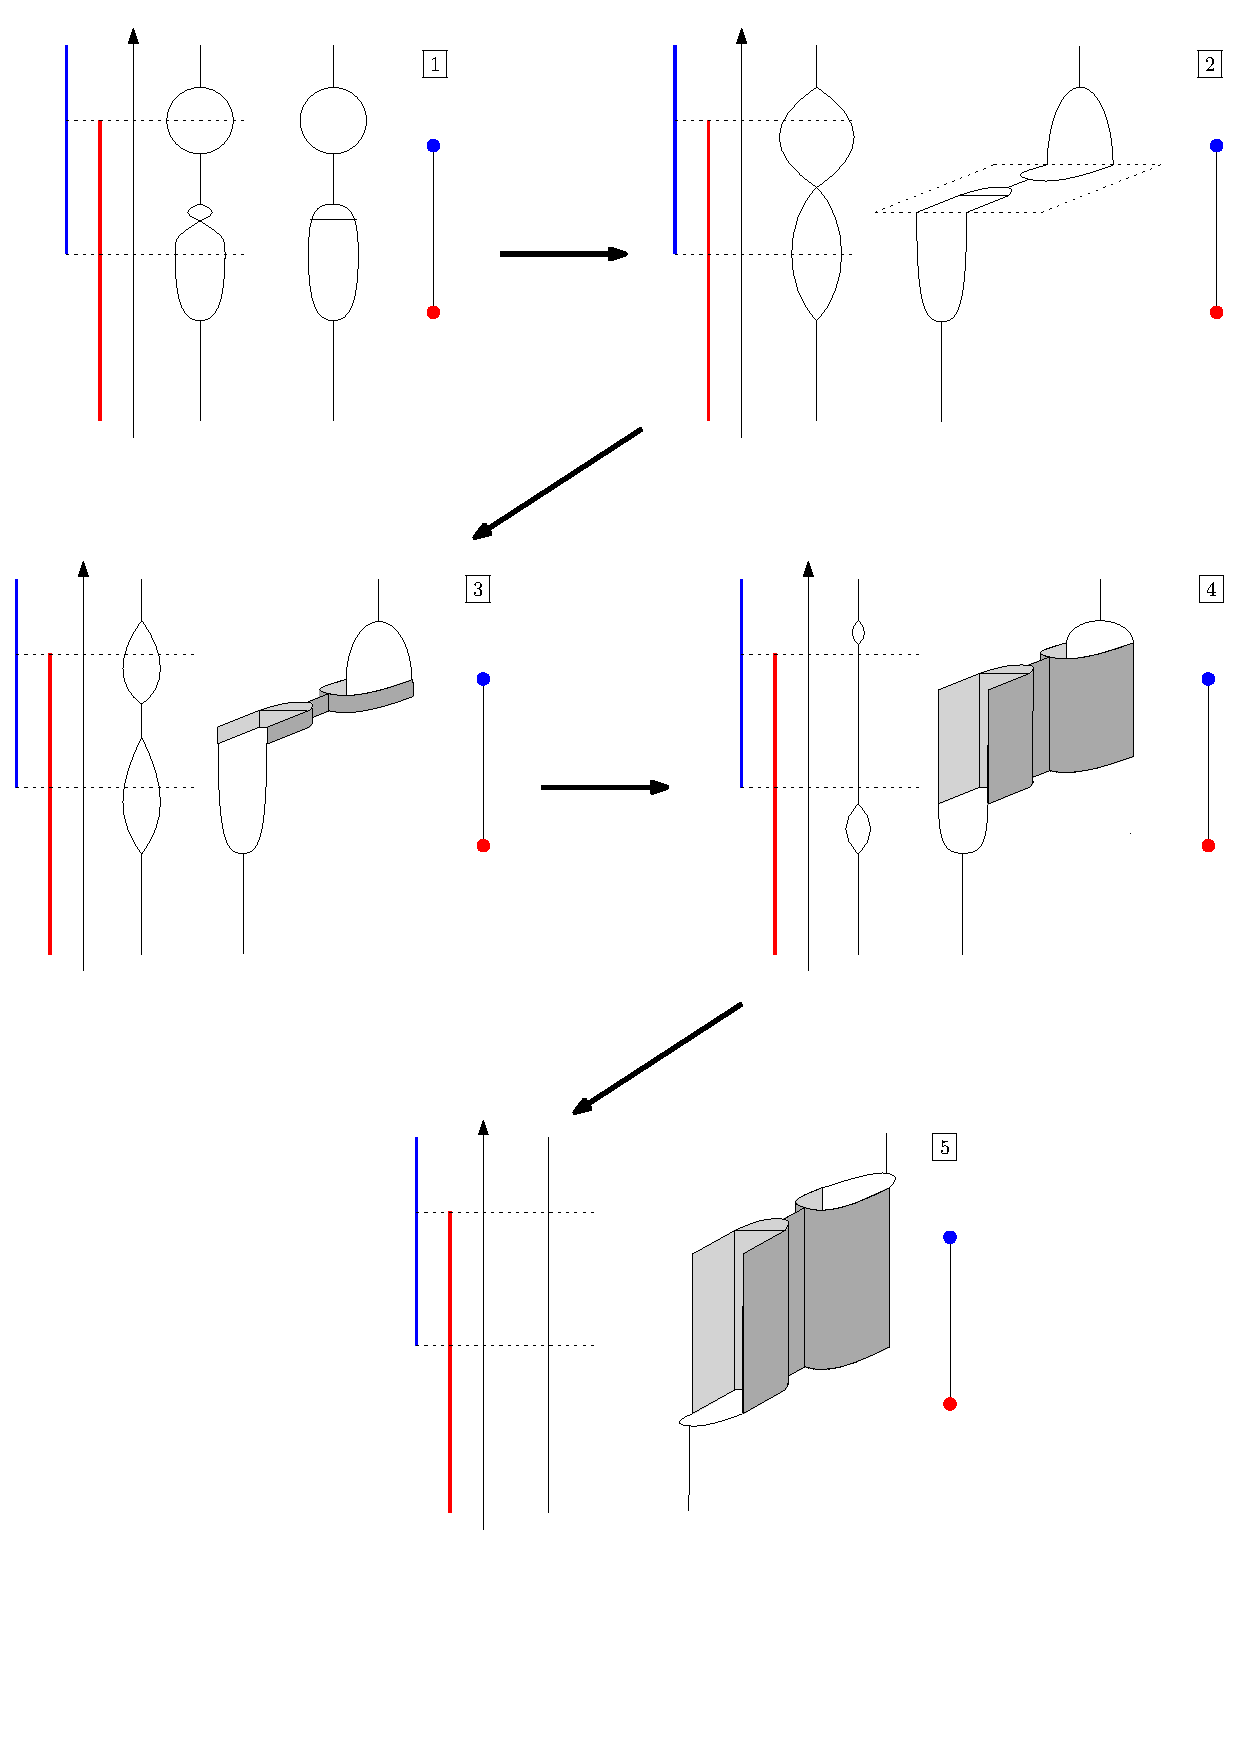
\includegraphics[width=12cm]{figures/Summary}
\caption[Full transformation on spaces]{\label{fig:summary} Illustration of the sequence of
  transformations in~(\ref{eq:final_transf}) on the features located in an interval
  intersection. For each figure, we display the original space
  (middle), its Reeb graph (left) and its MultiNerve Mapper (right).}
\end{center}
\end{figure}

\begin{lem}\label{lem:inv_Mapper}
For $(\MMtel,\fMMtel)$ defined as in Definition~\ref{eq:final_transf},
$\MMapper_{\fMMtel}(\MMtel,\I)$ and $\MMapper_f(X,\I)$ are isomorphic as combinatorial multigraphs.
\end{lem}



This allows us to prove the following result, which states that the MultiNerve Mapper $\MMapper_f(X,\I)$
is actually the same object than the perturbed Reeb graph $\Reeb_{\fMMtel}(\MMtel)$. 

\begin{thm}\label{th:Dg}
For $(\MMtel,\fMMtel)$ defined as in Definition~\ref{eq:final_transf}, $\MMapper_f(X,\I)$ and
$\mathcal{C}\Reeb_{\fMMtel}(\MMtel)$ are isomorphic as combinatorial multigraphs.
%Moreover, $\Dg(\tilde{f}')=\Dg(f_{\I})$, with $f_{\I}$ as in Definition~\ref{def:arbitfunc}.
\end{thm}
%
We know from Lemma~\ref{lem:inv_Mapper} that
$\MMapper_f(X,\I)$ and $\MMapper_{\fMMtel}(\MMtel,\I)$ are isomorphic as combinatorial multigraphs. Theorem~\ref{th:Dg} is 
then a consequence of the following result, whose hypothesis is satisfied by the~$\MMtel$ of
Definition~\ref{eq:final_transf}:
%
\begin{lem}\label{lem:MMapper-Reeb-isom} 
Let $T$ be a telescope and let $\pi_2:T\to\R$ be the projection onto the
second factor.  Suppose that every proper subinterval~$\tilde I$ in the
cover~$\I$ contains exactly one critical value of~$\pi_2$, and that the
intersections $I\cap J$ contain none. Then, $\MMapper_{\pi_2}(T,\I)$ and
$\mathcal{C}\Reeb_{\pi_2}(T)$ are isomorphic as combinatorial multigraphs.
\end{lem}
%
\begin{proof}
The nodes of $\mathcal{C}\Reeb_{\pi_2}(T)$ represent the connected components of the
preimages of all critical values of $\pi_2$, while the nodes of
$\MMapper_{\pi_2}(T,\I)$ represent the connected components of the preimages of all
$I\in\I$.  The hypothesis of the lemma implies that there is exactly
one critical value per interval $I\in\I$, hence the nodes of
$\MMapper_{\pi_2}(T,\I)$ and of $\mathcal{C}\Reeb_{\pi_2}(T)$ are in
bijection.  Meanwhile, the edges of $\mathcal{C}\Reeb_{\pi_2}(T)$
are given by the connected components of the $Y_i\times[a_i,a_{i+1}]$. Since the proper subintervals
contain one critical value each and the $I\cap J$ contain none, the
pullbacks of all intersections of consecutive intervals also span the
$Y_i\times[a_i,a_{i+1}]$. Hence, the edges of $\MMapper_{\pi_2}(T,\I)$
are in bijection with the ones of
$\mathcal{C}\Reeb_{\pi_2}(T)$. Moreover, their endpoints are defined
in both cases by the $\phi_i$ and $\psi_i$. Hence the multigraph
isomorphism.
\end{proof}

In passing, it is interesting to study the behavior of the MultiNerve
Mapper as the hypothesis of the lemma is weakened. For instance:
%
\begin{lem}\label{lem:MMapper-Reeb-quasi-isom} 
Let $T$ be a telescope and let $\pi_2:T\to\R$ be the projection onto
the second factor.  Suppose that every interval~$I$ in the cover~$\I$
contains at most one critical value of~$\pi_2$. Then, $\MMapper_{\pi_2}(T,\I)$
is obtained from $\mathcal{C}\Reeb_{\pi_2}(T)$ by splitting some
vertices into two and by subdividing some edges once.
\end{lem}
%
Thus, the MultiNerve Mapper may non longer be `exactly' isomorphic to
the combinatorial Reeb graph (counter-examples are easy to build, by
making some of the critical values fall into intersections of
intervals in the cover), however it is still isomorphic to it up to
vertex splits and edge subdivisions, which are
topologically trivial modifications.  
%
\begin{proof}[Proof of Lemma~\ref{lem:MMapper-Reeb-quasi-isom}]
The proof is constructive and it proceeds in 3 steps:

\noindent 1. For every interval $I\in\I$ that does not contain a
critical value, add a dummy critical value (with identities as
connecting maps) in the proper subinterval $\tilde I$. The effect on the
Mapper is null, while the effect on the Reeb graph is to subdivide once
each edge crossing the dummy critical value. At this stage, every
interval of $\I$ contains exactly one critical value. For simplicity
we identify $T$ with the new telescope.

\noindent 2. For every interval $I\in\I$ whose corresponding critical
value does not lie in the proper subinterval $\tilde I$ but rather in some
intersection $I\cap J$ (defined uniquely since $\I$ is a gomic), merge
$I$ and $J$ into a single interval $I\cup J$. The coarser cover
$\J$ thus obtained is still a gomic and it has the extra property that
every proper subinterval contains exactly one critical
value and every intersection contains none. Then, by
Lemma~\ref{lem:MMapper-Reeb-isom}, the MultiNerve Mapper
$\MMapper_{\pi_2}(T,\J)$ is isomorphic to the combinatorial Reeb graph
$\mathcal{C}\Reeb_{\pi_2}(T)$.

\noindent 3. There remains to study the differences between
$\MMapper_{\pi_2}(T,\I)$ and $\MMapper_{\pi_2}(T,\J)$. The only
difference between the two covers is that some isolated pairs of
intervals $(I,J)$ have been merged because their intersection $I\cap
J$ contained a critical value $a_i$. For every such pair, there are as
many connected components in the preimage $\pi_2^{-1}(I)$ as in $\pi_2^{-1}(J)$ as in
$\pi_2^{-1}(I\cap J)$ as in $\pi_2^{-1}(I\cup J)$ because $I\cup J$ contains
no critical value other than $a_i$. Hence, every vertex of
$\MMapper_{\pi_2}(T,\J)$ corresponding to a connected component of $\pi_2^{-1}(I\cup J)$
is split into two in $\MMapper_{\pi_2}(T,\I)$. Moreover, the two
copies are connected by a single edge, given by the corresponding connected component
of $\pi_2^{-1}(I\cap J)$. Now, assuming without loss of generality that
$J$ lies above $I$, we have $(I\cup J)_\cap^+=J_\cap^+$, which by
assumption contains no critical value, so the connections between the
vertex copy corresponding to $\pi_2^{-1}(J)$ and the vertices lying above
it in $\MMapper_{\pi_2}(T,\I)$ are the same as the connections between
the original vertex and the vertices lying above it in
$\MMapper_{\pi_2}(T,\J)$. Similarly, $(I\cup J)_\cap^-=I_\cap^-$
contains no critical value by assumption, so the connections between
the vertex copy corresponding to $\pi_2^{-1}(I)$ and the vertices lying
below it in $\MMapper_{\pi_2}(T,\I)$ are the same as the connections
between the original vertex and the vertices lying below it in
$\MMapper_{\pi_2}(T,\J)$.
\end{proof}

\paragraph*{Extension to the Mapper.} Due to the simple relation between the Mapper and the MultiNerve Mapper
given by Corollary~\ref{cor:projMNonM}, Theorem~\ref{th:Dg} can be extended for Mappers. 

\begin{defin}\label{cor:finaltransfMapper}
Let $X$ be a topological space, and $f:X\rightarrow\R$ be a Morse-type function. 
%with critical values $a_0=-\infty,a_1,\cdots,a_n,a_{n+1}=+\infty$.
Let $(\MMtel,\fMMtel)$ be defined as in Definition~\ref{eq:final_transf}.
Let ${\rm Cyl}(\MMtel)$ be the set of the connected components of the cylinders of $\MMtel$. 
We define the equivalence relation
$\sim$ between elements of ${\rm Cyl}(\MMtel)$ as: $$C\sim C'\Leftrightarrow \left\{\begin{array}{l} C,C'\text{ are connected components of the same cylinder} \\ 
\phi_i(C\times\{a_i\})\text{ and }\phi_i(C'\times\{a_i\})\text{ belong to the same connected component}\\
\psi_i(C\times\{a_{i+1}\})\text{ and }\psi_i(C'\times\{a_{i+1}\})\text{ belong to the same connected component} \end{array}\right.$$
Then, we define $\Mtel$ as $\MMtel/\sim$, equipped with the projection onto 
the second factor that we call $\fMtel$.
\end{defin}

Intuitively, we glue the pairs $C,C'$ of connected components of the same cylinder whose images under the attaching maps are in the same connected component of the critical slice, 
i.e. those that induce edges with the same endpoints in the multinerve. Hence, we obtain the following corollary using Corollary~\ref{cor:projMNonM}:

\begin{cor}\label{cor:transfMapper}
$\mathcal C\Reeb_{\fMtel}(\Mtel)$ and $\Mapper_f(X,\I)$ are isomorphic as combinatorial multigraphs.   
\end{cor}

%for which $\im(\phi_i|_{C\times\{a_i\}})=\im(\phi_i|_{C'\times\{a_i\}})$ 
%and $\im(\psi_i|_{C\times\{a_i\}})=\im(\psi_i|_{C'\times\{a_i\}})$.
%This gives a second telescope $T''_X$, which is equipped with the projection onto the second factor $\pi_2''$ that we rename $f''$,
%and whose combinatorial Reeb graph $\Reeb_{f''}(T''_X)$ is isomorphic to $\Mapper_f(X,\I)$.
    










\subsection{Convergence results.}
\label{sec:dfdconv}

Recall that the $\distfd$ compares metric graphs, whereas the (MultiNerve) Mappers
are combinatorial graphs.
However, since $\MMapper_f(X,\I)$ and $\Reeb_{\fMMtel}(\MMtel)$ are essentially the same according to Theorem~\ref{th:Dg},
we can use $\Reeb_{\fMMtel}(\MMtel)$ as a metric graph representation of $\MMapper_f(X,\I)$,   
when computing the functional distortion distance.
Note that we could also use $\Reeb_{\fMM}(\MMapper_f(X,\I))$ since it is isomorphic to $\MMapper_f(X,\I)$ as well according to Lemma~\ref{lem:idemMapper},
but its connection to $\Reeb_f(X)$ is unclear. %so we rather use $\Reeb_{\fMMtel}(\MMtel)$, whose connection to $\Reeb_f(X)$ is given by Definition~\ref{eq:final_transf}.
On the opposite, even though $\distfd$ is most of the time untractable, its computation is possible with $\Reeb_{\fMMtel}(\MMtel)$
thanks to the sequence of transformations of Definition~\ref{eq:final_transf}.
We will see at the end of the section that $\fMM$ and $\fRMMtel$ actually coincide on $\MMapper_f(X,\I)$.

Theorem~\ref{th:dfd} below shows that $\Reeb_{\fMM}(\MMapper_f(X,\I))$ is close to $\Reeb_f(X)$ if $\I$ has a small granularity. To prove it,
we use the following lemma, whose proof is just a simple extension of the one of Proposition~\ref{prop:fdb}:
%and is detailed in~\cite{Carriere15c}: %deferred to Appendix~\ref{sec:proof_dfd}:

\begin{lem}\label{lem:dfdmerge}
Let $S$ be a set of pairwise disjoint bounded open intervals, and let $\Merge_S$ be defined as
the composition of all $\Merge_{a,b}$, $(a,b)\in S$. 
Let $\Reeb_g$ be a Reeb graph such that $\Crit(\tilde g)\subset \bigcup_{I\in S} I$
and let $\Reeb_{g'}$ be the Reeb graph
of the telescope $\Merge_S(\Reeb_g)$.
Then $\distfd(\Reeb_g,\Reeb_{g'})\leq \sup\{{\rm length}(I)\,:\,I\in S\}$.
\end{lem}

Given a gomic $\I$, we let $\epsilon_1(\I)=\sup\{{\rm length}(\tilde I)\,:\,I\in\I\}$ and
$\epsilon_2(\I)=\sup\{{\rm length}(I\cap J)\,:\,I,J\in\I\}$. 
Note that $\epsilon_1(\I)$ and $\epsilon_2(\I)$ can be thought of as different types of granularity measures of $\I$.
They are both bounded from above by the granularity of $\I$ as defined in Section~\ref{sec:basicdef}. 

\begin{thm}\label{th:dfd}
Suppose the granularity of the gomic~$\I$ is at most $\e$.
For $(\MMtel,\fMMtel)$ defined as in Definition~\ref{eq:final_transf}, we have
$\distfd(\Reeb_{\fMMtel}(\MMtel),\Reeb_f(X))\leq \epsilon_1(\I)+\epsilon_2(\I)+\max\{\epsilon_1(\I),\epsilon_2(\I)\}\leq 3\epsilon$.

Moreover, for $(\Mtel,\fMtel)$ defined as in Definition~\ref{cor:finaltransfMapper}, we have
$\distfd(\Reeb_{\fMtel}(\Mtel),\Reeb_f(X))\leq 7\e/2$.
\end{thm}

\begin{proof}
%Recall that $\Reeb_{f'}(T_X')$ is obtained from $\Reeb_f(X)$ through the transformation~(\ref{eq:final_transf}).
We start with the MultiNerve Mapper.
By the triangle inequality, it suffices to bound the functional distortion distance for each of the four operations $\Merge_{\I}$,
$\Shift_{\I}$, $\Split_{\I}$ and $\Merge'_{\I}$ individually.
Let $\Reeb_1$ be the Reeb graph of the telescope $\Merge_{\I}(\Reeb_f(X))$.
Similarly, let $\Reeb_2$ be the Reeb graph of $\Split_{\I}(\Reeb_1)$, $\Reeb_3$ be the Reeb graph of $\Shift_{\I}(\Reeb_2)$ 
and $\Reeb_4=\Reeb_{\fMMtel}(\MMtel)$ be the Reeb graph of $\Merge'_{\I}(\Reeb_3)$. Examples of such Reeb graphs can be seen in the left
parts of Figure~\ref{fig:summary}.

Then we have
$\distfd(\Reeb_{\fMMtel}(\MMtel),\Reeb_f(X))\leq \distfd(\Reeb_f(X),\Reeb_1)+\distfd(\Reeb_1,\Reeb_2)+\distfd(\Reeb_2,\Reeb_3)+\distfd(\Reeb_3,\Reeb_4)$.

\begin{itemize}

\item By Lemma~\ref{lem:dfdmerge}, we have $\distfd(\Reeb_f(X),\Reeb_1)\leq \max\{\epsilon_1(\I),\epsilon_2(\I)\}$
and $\distfd(\Reeb_3,\Reeb_4)\leq \epsilon_1(\I)$.

\item Assume without loss of generality that $\Split_{\I}$ is the composition of all $\Split_{\alpha,\bar a}$, 
where $\bar a$ is a critical value of $\Reeb_1$. 
Since $\Reeb_1$ is obtained from $\Reeb_2$ by taking the composition of all $\Merge_{\bar a - \alpha,\bar a + \alpha}$,
it follows from Lemma~\ref{lem:dfdmerge} that $\distfd(\Reeb_1,\Reeb_2)\leq 2\alpha$.

\item Since the assumptions of Prop.~\ref{prop:MNInv}~(iii) and Prop.~\ref{prop:MNInv}~(iv) are satisfied by $\Shift_{\I}$,
it follows that $\Reeb_2$ and $\Reeb_3$ are isomorphic, because the number, the types and the ordering of the critical values of $\Reeb_2$
are preserved when transformed into $\Reeb_3$. It is then straightforward that the functional distortion distance between
$\Reeb_2$ and $\Reeb_3$ is the maximal amplitude of the $\Shift$ operations involved. According to the assumptions 
of Proposition~\ref{prop:MNInv}~(iii) and Proposition~\ref{prop:MNInv}~(iv),
these amplitudes are all bounded by $\epsilon_2(\I)$.

\end{itemize}

The result follows by letting $\alpha \rightarrow 0$.

Concerning the Mapper, the result is obtained by adding an extra $\epsilon/2$ to the previous upper bound,
which corresponds to the functional distortion distance cost of gluing edges with the same endpoints. %in $\Reeb_{f'}(T_X')$.
\end{proof}

Note that a similar result can be obtained directly by using the convergence result of the so-called 
{\em interleaving distance}---see Theorem 4.1 in~\cite{Munch16},
and the strong equivalence between the functional distortion distance and this interleaving distance---see Theorem 14 in~\cite{Bauer15}.
However, the upper bound gets larger ($7\epsilon$) and there is no clear intuition on the Reeb graph used to represent the Mapper 
(also called geometric Mapper) in~\cite{Munch16}.

Finally, Theorems~\ref{th:dfd} and~\ref{th:dfdstab} allow us to derive the following result with the triangle inequality:

\begin{cor} Let $X$ be a topological space, and
let $f,g:X\rightarrow\R$ be two Morse-type functions with continuous sections.
Let $(\MMtel(X,f),\fMMtel)$ (resp. $(\MMtel(X,g),\bar{g}_{\I})$) denote the pair computed with function $f$ (resp. $g$) as in Definition~\ref{eq:final_transf}.
%Let $(T'_X^f,f')$ and $(T'_X^g,g')$ defined as in Definition~\ref{eq:final_transf}.
Finally, let $\I$ be a gomic of granularity at most $\epsilon$. Then:
$$\distfd(\Reeb_{\fMMtel}(\MMtel(X,f)),\Reeb_{\bar{g}_{\I}}(\MMtel(X,g)))\leq \|f-g\|_\infty + 6\epsilon.$$
Moreover, for $(\Mtel(X,f),\fMtel)$ and $(\Mtel(X,g),g_{\I})$ computed as in Definition~\ref{cor:finaltransfMapper}, we have:
$$\distfd(\Reeb_{\fMtel}(\Mtel(X,f)),\Reeb_{g_{\I}}(\Mtel(X,g)))\leq \|f-g\|_\infty + 7\epsilon.$$
\end{cor}


%The proof of this result is a straightforward adaptation of the proof of Proposition~3.1 in~\cite{Carriere17a}.
%We provide it in Appendix~\ref{sec:proof_dfd} for completeness.
%\paragraph*{Extension to the Mapper.} Again, %Due to the simple relation between the Mapper and the MultiNerve Mapper, 
%Theorem~\ref{th:dfd} can be extended for the Mapper.
%
%
%Since the functional distortion distance is hard to compute and to interprete, making it difficult to use in practice,
%we rather focus on the bottleneck distance between the signatures in the remaining sections of this article,
%even though it is only a pseudometric.
%Note however that the bottleneck distance is actually locally equivalent to $\distfd$ for Reeb graphs~\cite{Carriere17a}.
%
%\paragraph{Stability.} 


\subsection{An alternative proof of Theorem~\ref{th:ExDgMultiNerve}}
\label{sec:alternateproof}

%%%
\begin{figure}[h]
\begin{center}
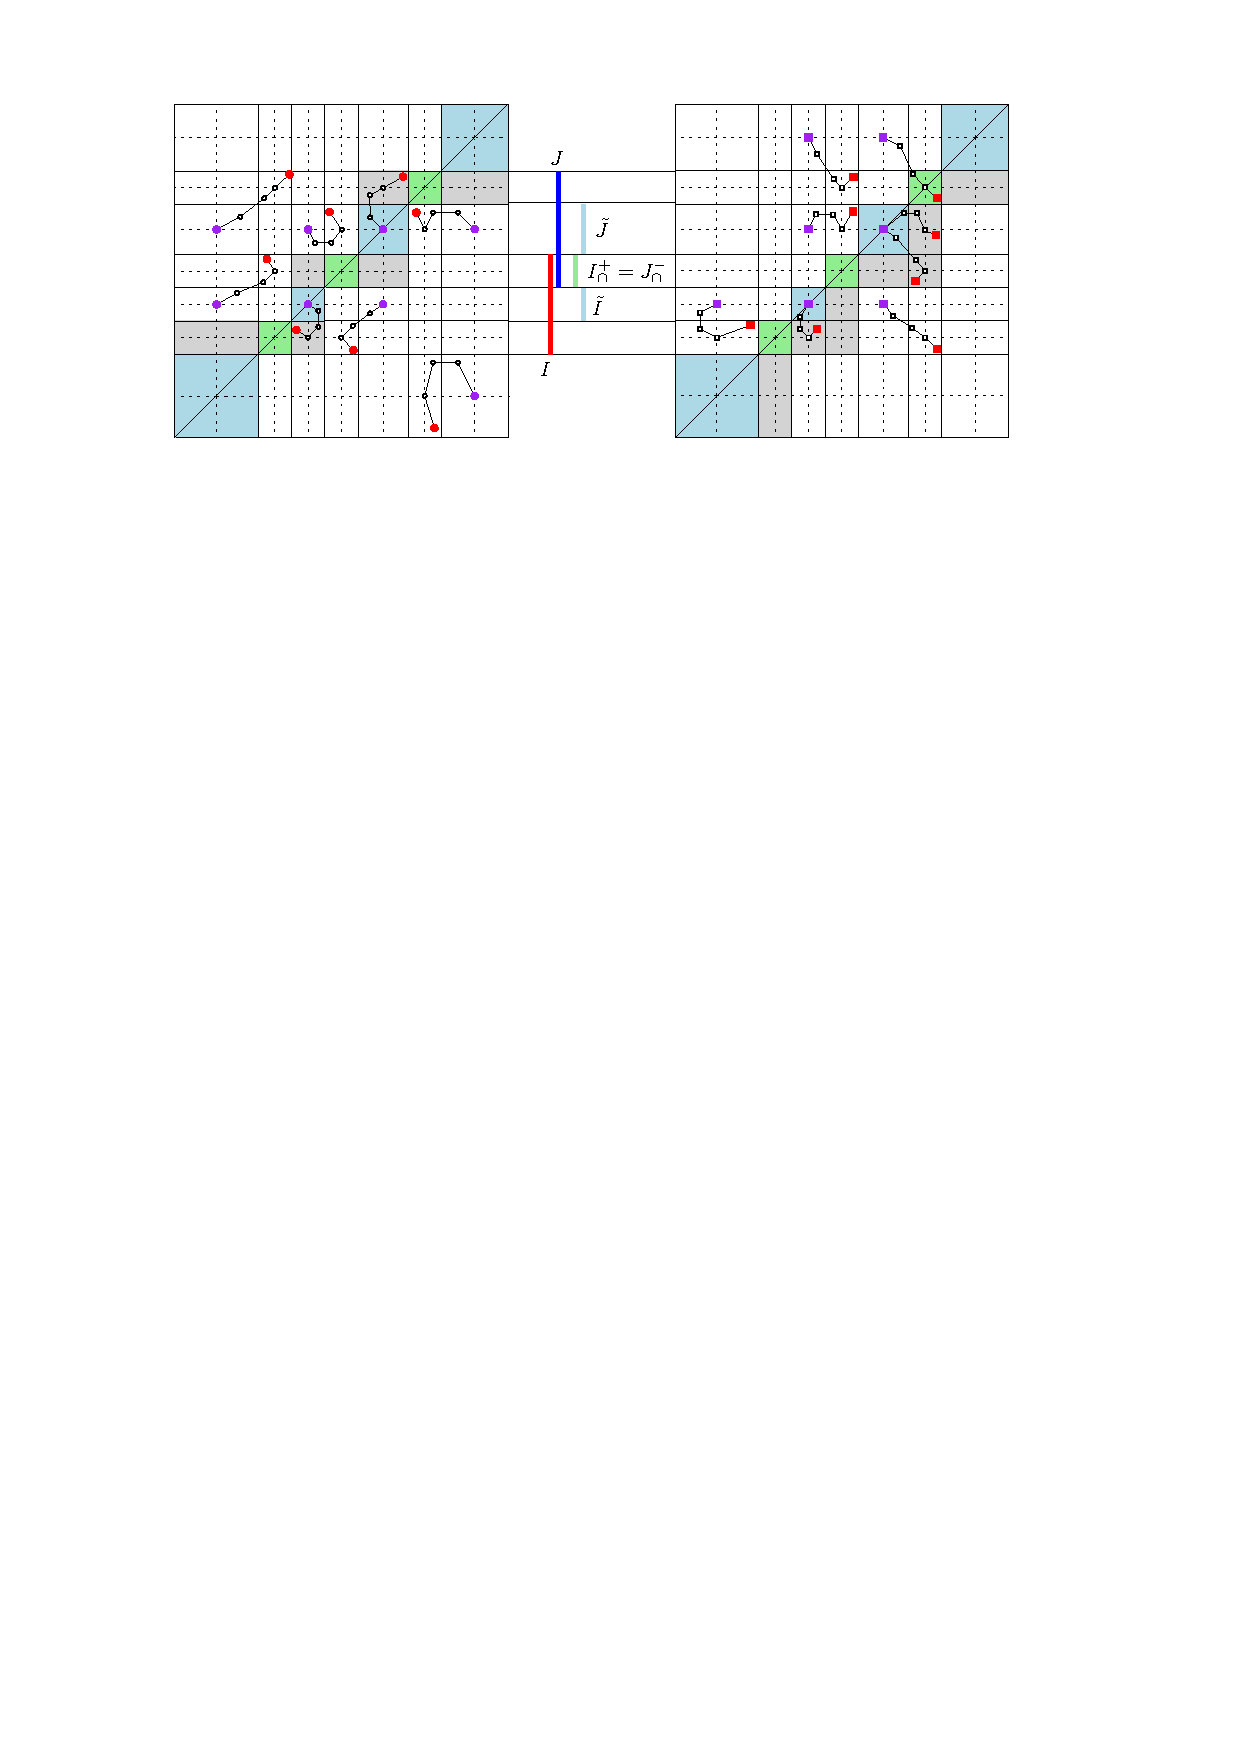
\includegraphics[width=14cm]{figures/FullTransformPD}
\caption[Full transformation on persistence diagrams]{\label{fig:pdTRANS}
The left panel displays
the trajectories of points in $\Ord$ (disks above the diagonal) and $\Rel$ (disks below the diagonal) while
the right panel displays the trajectories of points in $\Ext$.
For both diagrams, the original point is red, the final point is purple, and intersections and proper subintervals are colored
in green and light blue respectively. 
%Note that it is possible to build a pair $(X,f)$ that has exactly the PDs with the red points.
}
\end{center}
\end{figure}

We can prove Theorem~\ref{th:ExDgMultiNerve} again by studying the effect of 
the transformation defined in Definition~\ref{eq:final_transf} on the extended persistence
diagram of~$f$. These effect is illustrated in
Figure~\ref{fig:pdTRANS}.  There are two grids in this figure: the one
with solid lines is defined by the interval endpoints, while the one
with dotted lines is defined by midpoints of proper subintervals and intersections.  In the following, we
use the term \textit{cell} to designate a rectangle of the first grid.
Cells are closed if they correspond to proper subintervals for both
coordinates, they are open if they correspond to intersections for
both coordinates, and they are neither closed nor open otherwise.
Blue and green cells in Figure~\ref{fig:pdTRANS} correspond to squares
associated to a proper subinterval (blue) or intersection (green). We
can now interpret the effects of the transformations
in~(\ref{eq:final_transf}) on the persistence diagram visually:
%
\begin{itemize}
\item $\Merge_{\I}$ snaps all the points to the second grid by
  Lemma~\ref{lem:mergeprop}.
%
\item $\Split_{\I}$ moves the points 
to one of the four possible quarters inside their cell, 
depending on the point's type by Lemma~\ref{lem:splitprop}.
More precisely, ordinary points are moved to the down-left quarter,
extended points are moved to the up-left quarter, and relative points are moved to the up-right quarter.
%
\item Then, $\Shift_{\I}$ moves the points to a neighboring cell by Lemma~\ref{lem:shiftprop}.
% and the definition of $\Shift_\I$.
This neighboring cell is given by the point's type (as in the case of
$\Split_{\I}$) and by the coordinates of the point.  For instance, an
extended point $(x,y)$ lying in the row of a green cell and in the
column of another green cell, has coordinates that both belong to
interval intersections.
%: $x\in (I\cap J)$, $y\in I'\cap J'$. 
Then, this point is moved to the upper-left neighboring
cell. Differently, an extended point whose abscissa (resp. ordinate)
is in an intersection and whose ordinate (resp. abscissa) is not, is
only moved to the left (resp. upper) cell.  The same can be said for
ordinary (resp. relative) points by changing up-left to down-left
(resp. up-right).  Points whose coordinates both belong to proper
subintervals
%-- or, equivalently, whose cell is in the row of a blue cell and in the column of another blue cell --
are not moved by $\Shift_{\I}$, regardless of their type.
%
\item Finally, $\Merge'_{\I}$ re-snaps the points to the second grid by Lemma~\ref{lem:mergeprop}.
\end{itemize}
%
Thus, each point of $\Dg(f)$ can be tracked through the successive
operations of~(\ref{eq:final_transf}), and this tracking leads to the
following elementary observations:
%
\begin{enumerate}
\item The points of $\Ord(f)$ or $\Rel(f)$ that end their course on
  the diagonal after the sequence of
  operations of Definition~\ref{eq:final_transf} disappear in $\Dg(\fMMtel)$. This is
  because ordinary and relative points cannot be located on the
  diagonal. The rest of the points of $\Ord(f)$ or $\Rel(f)$ are
  preserved with the same type in $\Dg(\fMMtel)$.
\item Differently, all the points of $\Ext(f)$ are preserved with the
  same type ($\Ext$) in $\Dg(\fMMtel)$. However, some of the points of
  $\Ext^-(f)$ may end their course on or across the diagonal after the
  sequence of operations~(\ref{eq:final_transf}), thus switching from
  $\Ext^-(f)$ to $\Ext^+(\fMMtel)$. 
  %Their corresponding homology classes switch from vertical to horizontal.
\item All the points lie in the rows and columns of blue cells after
  $\Shift_{\I}$. Therefore, the points that end their course on the diagonal after
  the sequence of operations of Definition~\ref{eq:final_transf} are the ones
  located in blue cells after $\Shift_{\I}$.
\item Since transfers between cells occur only during $\Shift_{\I}$, a
  point $p$ that is not in a blue or green cell initially ends up in a
  blue cell~$B$ after $\Shift_{\I}$ if and only if:
\begin{itemize}
	\item $p$ is extended and it is in the down, right, or
          down-right neighboring cell of $B$ (grey cells in the right
          diagram of Figure~\ref{fig:pdTRANS}), or
	\item $p$ is ordinary and it is in the up neighboring cell of
          $B$ (grey cells above the diagonal in the left diagram of
          Figure~\ref{fig:pdTRANS}), or
	\item $p$ is relative and it is in the down neighboring cell
          of $B$ (grey cells below the diagonal in the left diagram
          of Figure~\ref{fig:pdTRANS}).
\end{itemize}
\item Points that belong to a blue or green cell initially are snapped
  to the diagonal by $\Merge_{\I}$. Among them, those that
  belong to a blue cell stay there until the end, whereas those that
  belong to a green cell eventually leave it---they end up in a blue
  cell after $\Shift_{\I}$ if they are ordinary or relative, while they end
  up in a white cell above the diagonal if they are extended.
%\item Points that belong to blue cells after $\Shift_\I$ are snapped to the diagonal by the second $\Merge_\I$.  
\end{enumerate}
%
The outcome of these observations is the following one. Observations 1, 3,
4, 5 imply that the points of $\Ord(f)$ that disappear in $\Dg(\fMMtel)$
are the ones located initially in the staircase made of
the blue, green and grey areas above the diagonal in the left
panel of Figure~\ref{fig:pdTRANS}, which is nothing but~$Q_O^{\I}$. 
Similarly, the points of $\Rel(f)$
that disappear in $\Dg(\fMMtel)$ are the ones located initially in the
staircase made of the blue, green and grey areas below the
diagonal in the left panel of Figure~\ref{fig:pdTRANS}, which is nothing but~$Q_R^{\I}$. 
Finally, observations 2, 3, 4, 5 imply that the points of $\Ext^-(f)$ that
switch to $\Ext^+(\fMMtel)$ are the ones located initially in the
staircase made of the blue, green and grey areas below the
diagonal in the right panel of Figure~\ref{fig:pdTRANS}, which is nothing but~$Q_{E^-}^{\I}$. 
The rest of the points of $\Dg(f)$ are preserved (albeit shifted) with the same type ($\Ord$,
$\Rel$, $\Ext^+$, $\Ext^-$) in $\Dg(\fMMtel)$. Hence, 
%the following result:
there is a perfect matching between:
\begin{center}
\begin{tabular}{ll}
{\rm (i)} $\Ord(\fMMtel)$ and $\Ord(f)\setminus Q_O^{\I}$ & 
{\rm (iii)} $\Ext^-(\fMMtel)$ and $\Ext^-(f)\setminus Q_{E^-}^{\I}$\\
{\rm (ii)} $\Rel(\fMMtel)$ and $\Rel(f)\setminus Q_R^{\I}$ &
{\rm (iv)} $\Ext^+(\fMMtel)$ and 
$\Ext^+(f) \cup (\Ext^-(f)\cap Q_{E^-}^{\I})$
%$\Ext_p^+(f) \cup (\Ext_p^-(f)\cap Q_{E^+}^\I)$
\end{tabular}
\end{center}

This, combined with Theorem~\ref{thm:pdreeb}, is equivalent to Theorem~\ref{th:ExDgMultiNerve}. %Note also that $\fMMtel$ and $\fMM$
This matching also shows that the critical points of $\fMMtel$ and $\fMtel$ are  located at the midpoints
of proper subintervals of the gomic's elements. Hence, $\fRMMtel$ and $\fRMtel$ actually coincide with $\fMM$ and $\fM$,
which allows us to state this final result:


\begin{thm}
\label{th:MultiNerveCover}
%Under the conditions stated at the beginning of the section,
Let $X$ be a topological space and $f:X\rightarrow\R$ be a Morse-type function. 
Let $\I$ be a gomic with granularity at most $\epsilon$.
Let $\fMM$ and $\fM$ be as in Definition~\ref{def:arbitfunc}. Then:
%For $(\MMtel,\fMMtel)$ defined as in Definition~\ref{eq:final_transf}, %for every $p\geq 0$
\begin{align}
\distb(\Dg(\fMM),\Dg(\tilde f))&\leq \epsilon /2,\label{eq:BottleIneqMMapperReeb} \\
%\end{equation}
%and %for $(\Mtel,\fMtel)$ defined as in Corollary~\ref{cor:finaltransfMapper},
%\begin{equation}
\distb(\Dg(\fM),\Dg(\tilde f))&\leq \epsilon.\label{eq:BottleIneqMapperReeb}
\end{align}
Moreover, in both cases, the matching achieving the distance %$\distb(\Dg(\tilde f'),\Dg(\tilde f))$ 
is actually a bijection preserving types. 
\end{thm}

 

%Even though we represent $\MMapper_f(X,\I)$ with $\Reeb_{f'}(T_X')$ because of Theorem~\ref{th:Dg},

%Equation~(\ref{eq:BottleIneqMapperReeb}) will be used to prove Theorem~\ref{thm:geomineq} in Chapter~\ref{chap:MapperStatistic}.
%This result is the main ingredient to show the rate of convergence of the Mapper to the Reeb graph. 

%Then, 
%and~\ref{th:MultiNerveCover} together 
%induces the following perfect matching between the persistence diagrams of the
%quotient maps:

%\vspace{-1.5pt}
%\begin{equation}\label{eq:matching_Dg_f-tilde}
%\Ord(\tilde f')\ \mbox{and}\ \Ord(\tilde f)\setminus Q_O^{\I}; \quad
%\Ext(\tilde f')\ \mbox{and}\ \Ext(\tilde f)\setminus Q_{E^-}^{\I}; \quad 
%\Rel(\tilde f')\ \mbox{and}\ \Rel(\tilde f)\setminus Q_R^{\I},
%\end{equation}

%which proves Theorem~\ref{th:ExDgMultiNerve} since $\Dg(\tilde f')=\Dg(f_{\I})$ by Theorem~\ref{th:Dg}.

%\paragraph*{Bottleneck distance.} The matching given by Figure~\ref{fig:pdTRANS} allows to bound the bottleneck distance $\distb$
%between $\Dg(f_{\I})$ and $\Dg(\tilde f)$.
%If the gomic $\I$ has granularity at most $\epsilon$, then
%\begin{equation}\label{eq:BottleIneqMapperReeb}
%\distb(\Dg(f_{\I}),\Dg(\tilde f))\leq \epsilon /2.
%\end{equation}

\section{Conclusion}

%\paragraph{Two different signatures.} 

In this chapter, we showed that the topological structure of the (MultiNerve) Mapper can be simply read off from the one
of the Reeb graph, via an appropriate simplification of its extended persistence diagram.
This simplification, namely the removal of points belonging to specific staircases, allowed us
to define a natural distance between (MultiNerve) Mappers by using appropriate signatures 
$\Dg(\MMapper_f(X,\I))$ and $\Dg(\Mapper_f(X,\I))$, to show that (MultiNerve) Mappers 
converge to their corresponding Reeb graphs (Corollary~\ref{cor:Reeb_approx}) and that they are stable (Theorem~\ref{thm:MStab}) with respect to this distance.
Moreover, we also showed that (MultiNerve) Mappers actually converge to their corresponding Reeb graphs
in the functional distortion distance, by using computable functions $\fMM$ and $\fM$ %defined on the (MultiNerve) Mappers 
(Theorem~\ref{th:dfd}).


Among the future perspectives of this work are the following questions:
\begin{itemize}

\item {\bf Does the local equivalence hold for Mapper?} In Chapter~\ref{chap:backgroundTelescopesReeb}, we showed that $\distb$ is locally a true metric for Reeb graphs.
Extending this result to Mappers would require to find an equivalent of $\distfd$ that depends on the gomic $\I$. 

\item {\bf Can our analysis be extended to multivariate function?} The main limitation of this work is to be restricted to scalar-valued functions, even though this is very common in applications.
The question whether our analysis can extend to multivariate functions $f:X\rightarrow\R^D$, with $D>1$, remains open, and
would require to extend the space's stratifications induced by Morse-type functions. A possible way to proceed is to study the so-called {\em Jacobi sets}
of multivariate functions~\cite{Chattopadhyay16, Edelsbrunner02a, Edelsbrunner08, Tierny17}, and to use recent results about 
decomposition of multidimensional persistence modules~\cite{Botnan16, Cochoy16}.  
\end{itemize}

%More precisely, we defined two different sets of signatures for (MultiNerve) Mappers with different properties, namely
%  and $\Dg(\fMM)$, $\Dg(\fM)$.
%The former, which depends only on the Reeb graph---thus canonical---but cannot be computed exactly,
%was used in Sections~\ref{sec:structure} and~\ref{sec:Stab_func} to 
%state convergence  and stability  in the bottleneck distance, while
%the latter, which is computable since it depends only on the gomic, but also instable since it is arbitrary, was used in Section~\ref{sec:stabdfd} to state
%convergence results in both the bottleneck (Theorem~\ref{th:MultiNerveCover}) and functional distortion distance   

%\bibliographystyle{plain}
%\bibliography{biblio}
